\documentclass[sigconf, anonymous]{acmart}

\fancyhf{} % Remove fancy page headers
\fancyhead[C]{Anonymous submission \#288 to ACM CCS 2017}
\fancyfoot[C]{\thepage}

\setcopyright{none} % No copyright notice required for submissions
\acmConference[Anonymous Submission to ACM CCS 2017]{ACM Conference on Computer and Communications Security}{Due 19 May 2017}{Dallas, Texas}
\acmYear{2017}

\settopmatter{printacmref=false, printccs=true, printfolios=true} % We want page numbers on submissions

\usepackage{listings}
\usepackage{amsmath}
\usepackage{amssymb}
\usepackage{mathtools}
\usepackage{url}

\DeclarePairedDelimiter{\ceil}{\lceil}{\rceil}
\newcommand{\overbar}[1]{\mkern1.5mu\overline{\mkern-1.5mu#1\mkern-1.5mu}\mkern 1.5mu}
\newcommand\defeq{\stackrel{\mathclap{\normalfont\mbox{def}}}{=}}

\begin{document}
\title{On the (in)security of encryption over compression in TLS}

\begin{abstract} When compression is composed with encryption, unexpected
vulnerabilities can arise. Such vulnerabilities have been explored in practical
attacks against TLS such as CRIME, TIME, and BREACH, even after TLS 1.3.
In this work we perform a thorough and systematic study of these attacks
and provide both practical and theoretical contributions.
First, motivated by the lack of production-grade testing tools, we provide Rupture, a
modular scalable open-source attack framework that implements
compression side-channel attacks in a robust manner. Second, we introduce an abstract
theoretical cryptographic model to express such attacks, the \textit{adaptive
reflection security} ``game''. Specifically, we
express \textit{compression idealness} and experimentally show that typical
compression functions exhibit partially ideal behavior. We then argue that
plaintext distributions used in practice follow an \textit{interdependent} joint distribution,
a stronger notion of dependent joint distributions. Based on these two
properties, we prove that \textit{compression-detectability} of predicates
arises, i.e. the ability to compute a predicate of the plaintext using
a reflection attack. Using this we demonstrate that {\em all}
length-preserving encryption schemes are insecure when composed with such
functions. Finally, we propose a novel defense protocol, \textit{context
hiding}, and provide an implementation of it, \textit{CTX}, that effectively
eliminates the threat these attacks pose with minimum performance and
deployment overhead. We argue about the security of our defense method based on
our model, as this technique modifies the plaintext joint distribution in
order to remove interdependence. We also demonstrate that CTX performs
significantly more favorably in terms of compression rate compared to previous
defense techniques.\end{abstract}


\begin{CCSXML}
    <ccs2012>
    <concept>
    <concept_id>10002978.10003022.10003026</concept_id>
    <concept_desc>Security and privacy~Web application security</concept_desc>
    <concept_significance>500</concept_significance>
    </concept>
    </ccs2012>
\end{CCSXML}

\ccsdesc[500]{Security and privacy~Web application security}

\keywords{compression, BREACH, CRIME, web security, defense, reflection security}

\maketitle

\section{Introduction}\label{sec:prev}

Compression and encryption composition has caused serious security problems in
protocols such as TLS \cite{dierks2008tls} over the years, with an array of
attacks making major headlines in computer security dissemination forums,
including BREACH \cite{gluck2013breach}, TIME \cite{be2013perfect}, and CRIME
\cite{duong2012crime}. Although the idea that compression is a side-channel that
can be exploited is certainly folklore in the cryptography community and is
documented at least as early as Kelsey's work \cite{kelsey2002compression}, a
proper theoretical model capturing the real-world perspective of these
side-channel attacks is still elusive.

Motivated by this, in this paper we introduce a general model that incorporates
the rendering process that is exploited during these attacks and facilitate a
thorough theoretical analysis of the security of encryption-compression
composition. We showcase the power of our approach by (i) demonstrating an
attack framework, called Rupture, that substantially improves the attack
performance, (ii) showing the above attacks can be expressed as instances
of our compression side-channel attack template, (iii) presenting a general
mitigation strategy, called context hiding, and our implementation of it called
CTX, that strikes a good balance between security and efficiency and can be
readily incorporated in a TLS system without a significant performance
degradation.

% More information on related work can be
%found on Appendix B.

\noindent
\textbf{Our contributions.} First, we implement Rupture,\footnotemark[1] an open
source production-grade framework for conducting compression and encryption
composition attacks. This generic framework provides an extensible mechanism for
experimentally testing attack techniques in a modular setting and we implement
the specific compression attack instance of BREACH. This is the first
time a working tool is provided for this class of attacks and an extensive
description of its architecture is in section \ref{app:rupture}.

Our attack framework achieves significant improvements compared to previous
attempts. We improve the complexity from linear to logarithmic in the secret's
alphabet size, attack block ciphers in addition to stream ciphers and employ
practical techniques for network level optimization. Our optimizations are
described in section \ref{subsec:optimizations} and experimental results are
offered in section \ref{subsec:rupture_experiments}.

We then introduce a model for analyzing compression and encryption composition
attacks, the \textit{adaptive reflection game}, with an accompanying security
definition, in section \ref{sec:refsec}. This model is novel as it generalizes
the concept and the properties of these attacks.

We prove that all encryption functions are insecure when composed with
compression, based on a series of required assumptions. We define the properties
\textit{interdependence} and \textit{compression idealness} and show that these
somewhat innocent properties enable the construction of an attacker, which we
prove breaks the security of the scheme.

Having established the attack premises, we shift our interest in defending
against such attacks. Although there are several proposed defenses, we feel that
none achieves good compression performance in real-world systems. In this
direction, section \ref{sec:defense} introduces \textit{context hiding}, a
method that mitigates a class of practical compression side-channel attacks like
BREACH.

Our implementation of the context hiding defense technique is called
CTX\footnote[1]{The GitHub repositories of the Rupture and CTX projects make the
source code openly available but have been removed for anonymization purposes
and can be provided upon request.}. CTX runs at the application layer of web
services, is opt-in, and achieves better balance between security and
compression performance compared to existing defense methods.

We experimentally show that CTX performs well in time and space. Specifically,
we find that the performance penalty of CTX compared to other proposed methods
is significantly lower and within accepted rates for real-world applications.

Finally, we provide theoretical arguments as to why CTX is an effective defense
method.

\section{Compression attacks}\label{sec:attack}

\subsection{A high-level overview}\label{subsec:example}
Compression side-channel attacks pose a serious threat
against TLS and any encryption system in general.
Although widely acknowledged and documented by the security community, there
still exist too few mitigation strategies to thwart them, primarily due to
(i) the perceived high performance penalty associated with mitigating them, and
(ii) the perceived complexity that results in a lack of production code tools to allow for
the robust execution of such attacks. In this work we illustrate that these
perceptions are wrong and the continuous existence of such realistic threats
suggests a grave situation that needs to be addressed.

In order to appreciate the seriousness of these attacks we begin a high-level
overview.

Suppose that a user browses the Internet and accesses a website, e.g. a social
network or a service that handles sensitive private data. When she requests a
page on this site, the server collects all needed data, generates the HTML code
age and sends a response over the network containing the page's code.  All response
data is encrypted under TLS, which ensures privacy and integrity for this
communication, and compressed for efficiency.

Consider now an adversary who aims to break this communication's security by
effectively revealing information about the exchanged private data. He decides
to mount a compression side-channel attack, so he must first make sure that
certain conditions are met.

Firstly, the adversary has a passive level of network access. That way he is
able to collect and analyze the network packets of the encrypted communication
with the server.

Secondly, he is able to issue any number of malicious requests using the user's
cookies (which will be encrypted). He can achieve this by forcing the user's
browser to run a piece of code, such as a Javascript script. This script will be
either hosted on an adversary-controlled website or injected in plain HTTP
responses from third websites, in which case the adversary also needs active
level of network access. When loaded in the user's browser, the script
can issue requests to any URL crafted by the adversary. Figure
\ref{fig:attack_model} elaborates on this attack mode.

Thirdly, the website under attack allows data injection in the encrypted
plaintext. This data takes the form of a specially crafted ``reflection'' string
that the adversary includes in the malicious requests. Depending on where the
targeted secret exists, the reflection need be included in either the
request, as is the case of CRIME which targets authentication cookies, or the
response plaintext, like the case of BREACH targeting CSRF tokens
\cite{de2011automatic}.

The adversary issues the attack in stages. In each stage he creates a pool of
reflections and makes malicious requests for each reflection in the pool.  As
the attack progresses the adversary collects network data related to multiple
requests and reflections.  Although this data is encrypted, analysis on the
packet lengths can reveal otherwise hidden properties of the private data.  An
attack stage ends when the adversary has successfully decrypted a single
character in the secret. We will elaborate on the form of the reflections and
the analysis in section \ref{subsec:rupture}.

At this point the privacy of the communication between the user and the website
has been compromised, since the adversary has broken the confidentiality of the messages
by effectively circumventing TLS security.

    \begin{figure}[thpb]
        \centering
            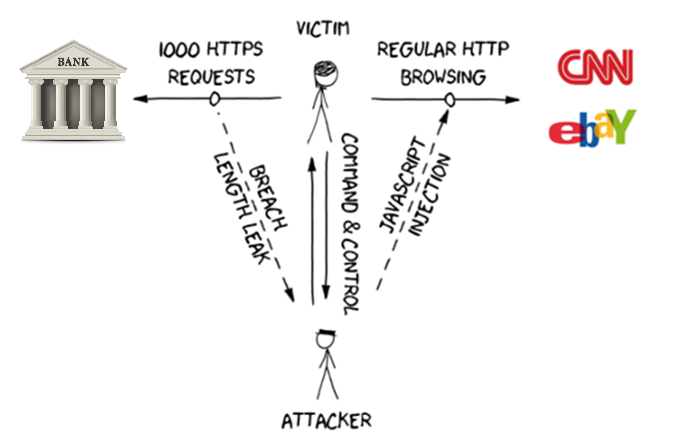
\includegraphics[width=0.48\textwidth]{figures/attack_model.png}
        \caption{The attack model}
        \label{fig:attack_model}
    \end{figure}

\subsection{A motivating example, concepts and notations}\label{subsec:terms}
We now describe a concrete example of the scenario in the previous section to
illustrate the various terms we use in the rest of this paper.

The target of the attack is a mail service found in the URL
\textit{mail.example.com}. The victim is a user that is logged in this service
and browses the Internet.

The web page that the adversary exploits is
\textit{\url{mail.example.com/search?query=attack}}. This page provides the HTTP
GET parameter \textit{query} and an example of a reflection that the adversary
uses is the string \textit{attack}. The HTML response for this request is:

\begin{lstlisting}[basicstyle=\small\ttfamily]
<div>
    <p>You searched for: attack</p>
    <p>No results found.</p>
</div>
<div>
    Your inbox:
    <ul>
    <li>[Bank] Routing number: 123</li>
    </ul>
</div>
\end{lstlisting}

Using the terms introduced in the following sections, the server's function
that generates the HTML code
is an instance of the \textit{rendering function} $f$. The output of $f$ is the
\textit{rendered message} $m$, in our example the HTML response.

The response contains multiple data elements. A data element can be a
\textit{secret}, \textit{static}, or a \textit{reflection}.

A \textit{secret} $s$ is any part of the response that the application wishes to
keep private. Examples of secrets include private messages, financial data, and
web security elements like CSRF tokens. In our example,
the strings ``Bank", which is an email topic, and ``Routing number: 123", which
is the email body, are both secrets.

\textit{Static} is any content that remains unchanged across requests.  Examples
of static data is HTML code, like ``div", or strings like ``Your inbox:" in our
example.  Static content is predictable and thus irrelevant to the attack.

A \textit{reflection} $r$ is a component crafted by the attacker that can be
adaptively transformed as the attack progresses. In this case, the HTTP GET
value ``attack" is a reflection. This string is included in the response in ``You
searched for: attack", an information message for the user used in every
search request.

Secrets are chosen from the distribution $\mathcal{M}$, which in this case
contains all routing numbers and 4-letter strings like ``Bank".

The compression function $\textrm{Com}$ is the compression algorithm used on the
HTML response plaintext. In our example, this algorithm is DEFLATE, the most
common compression algorithm on the web.

The encryption function $\textrm{Enc}$ is the encryption algorithm used by the
web server, the most common today being AES \cite{daemen2013design}. We use the function
$\mathcal{E}$ to describe the composition of $\textrm{Enc}$ and $\textrm{Com}$.

The input of $\mathcal{E}$ is the message $m$ and its output is the
ciphertext $c$ that is sent in the response packets and is sniffed by the
adversary over-the-wire.

\section{Rupture: An improved attack}\label{subsec:rupture}
Our first contribution is the development of a production-grade framework called
Rupture, which was developed as part of the work on extending the BREACH attack
against modern systems.

Rupture provides extended functionality regarding the network aspects of the
attack. It offers the ability to inject malicious code in any computer on the
network, perform traffic inspection and analyze captured data.

\subsection{Attack design}\label{subsec:rupture_attack_design}

Rupture enables the automated computation of the reflection strings in each
round of the attack. For this computation, the adversary should firstly know a
prefix of the secret, which is needed to build the initial reflections and
bootstrap the attack.

Each reflection consists of the known prefix concatenated with a character in
the candidate alphabet. The candidate alphabet initially is equal to the
alphabet of the secret and, as the attack progresses, it may be reduced to a
smaller set of symbols. This construction method ensures that a reflection $r_i$
in the reflection vector $\bar{r} = <r_1, r_2, ...>$ will match the secret.

The adversary issues consecutive requests, each containing a different
reflection. The goal is to recognize the one that matches secret, which is
achieved by exploiting the way most compression functions like DEFLATE behave.

In the case when $r$ matches the secret $s$, the compression will be better than
a case of no-match. Therefore, the network response packets for the matching
reflection will be smaller than the packets of the incorrect reflections.

We define a \textit{sample} as the encrypted data pertaining to one response for
a single reflection. The set of samples collected for a particular reflection is a
\textit{sampleset}. The collected samplesets for all candidates in the alphabet
form a \textit{batch}.

The attack is conducted in \textit{rounds}. In each round, a decision is made
about the state of the attack, so either the next byte of the secret becomes
known or the candidate alphabet is drilled down to a smaller set. Rupture
amplifies the results by using multiple samples in each
sampleset in order to achieve better probability of success. Therefore during the
analysis Rupture collects a batch's samplesets, compares the mean length of the
responses for all candidates, and chooses the candidate with the smaller mean
response length as the correct one.

This decision is made with some \textit{confidence} which is expressed in bytes.
If the confidence is insufficient, an additional batch is collected and the
analysis is redone using the aggregated lengths from all collected batches.

Once enough batches have been collected for a decision to be made with good
confidence, the round of the attack is complete.  Each stage of the attack
consists of one or more rounds and is concluded by decrypting a single byte of the
secret.

\subsection{Architecture}\label{app:rupture}
Rupture is a service-based architecture framework which contains multiple
independent components. The components are able to run on
different networks, although the attack can be easily launched by running all
modules on a single system.

The framework assumes a \textit{target} service to be attacked. This target is a
web service which uses TLS and provides HTTPS endpoints as described in section
\ref{subsec:example}. However, we have designed Rupture to be a good playground
for experimentation with new attacks, so this assumption can be relaxed and
attacks against other similar protocols are possible. Examples of other
encrypted protocols that can be explored in future work include SMTP and XMPP.

The framework also assumes the \textit{victim}, a user who is associated with
the particular target and whose data will be decrypted. Both the target and the
victim are modeled with various attributes and are easily configurable.

There are two underlying assumptions in our attack: the injection and the
sniffing. These are often, but not necessarily, achieved through the same means.
The injection assumption states that the adversary is able to inject code, the
\textit{client}, to the victim's machine for execution. This code is able to
issue adaptive requests to the target service. The sniffing assumption states
that the adversary is able to observe encrypted network traffic between the
victim and the target. Although a passive network access for the adversary
covers the sniffing assumption, in the cases where injection is needed the
adversary should have active network access.

Rupture's architecture is depicted in figure \ref{fig:rupture_architecture} and
the various components that implement the above are described in detail in the
following paragraphs.

   \begin{figure}[thpb]
      \centering
          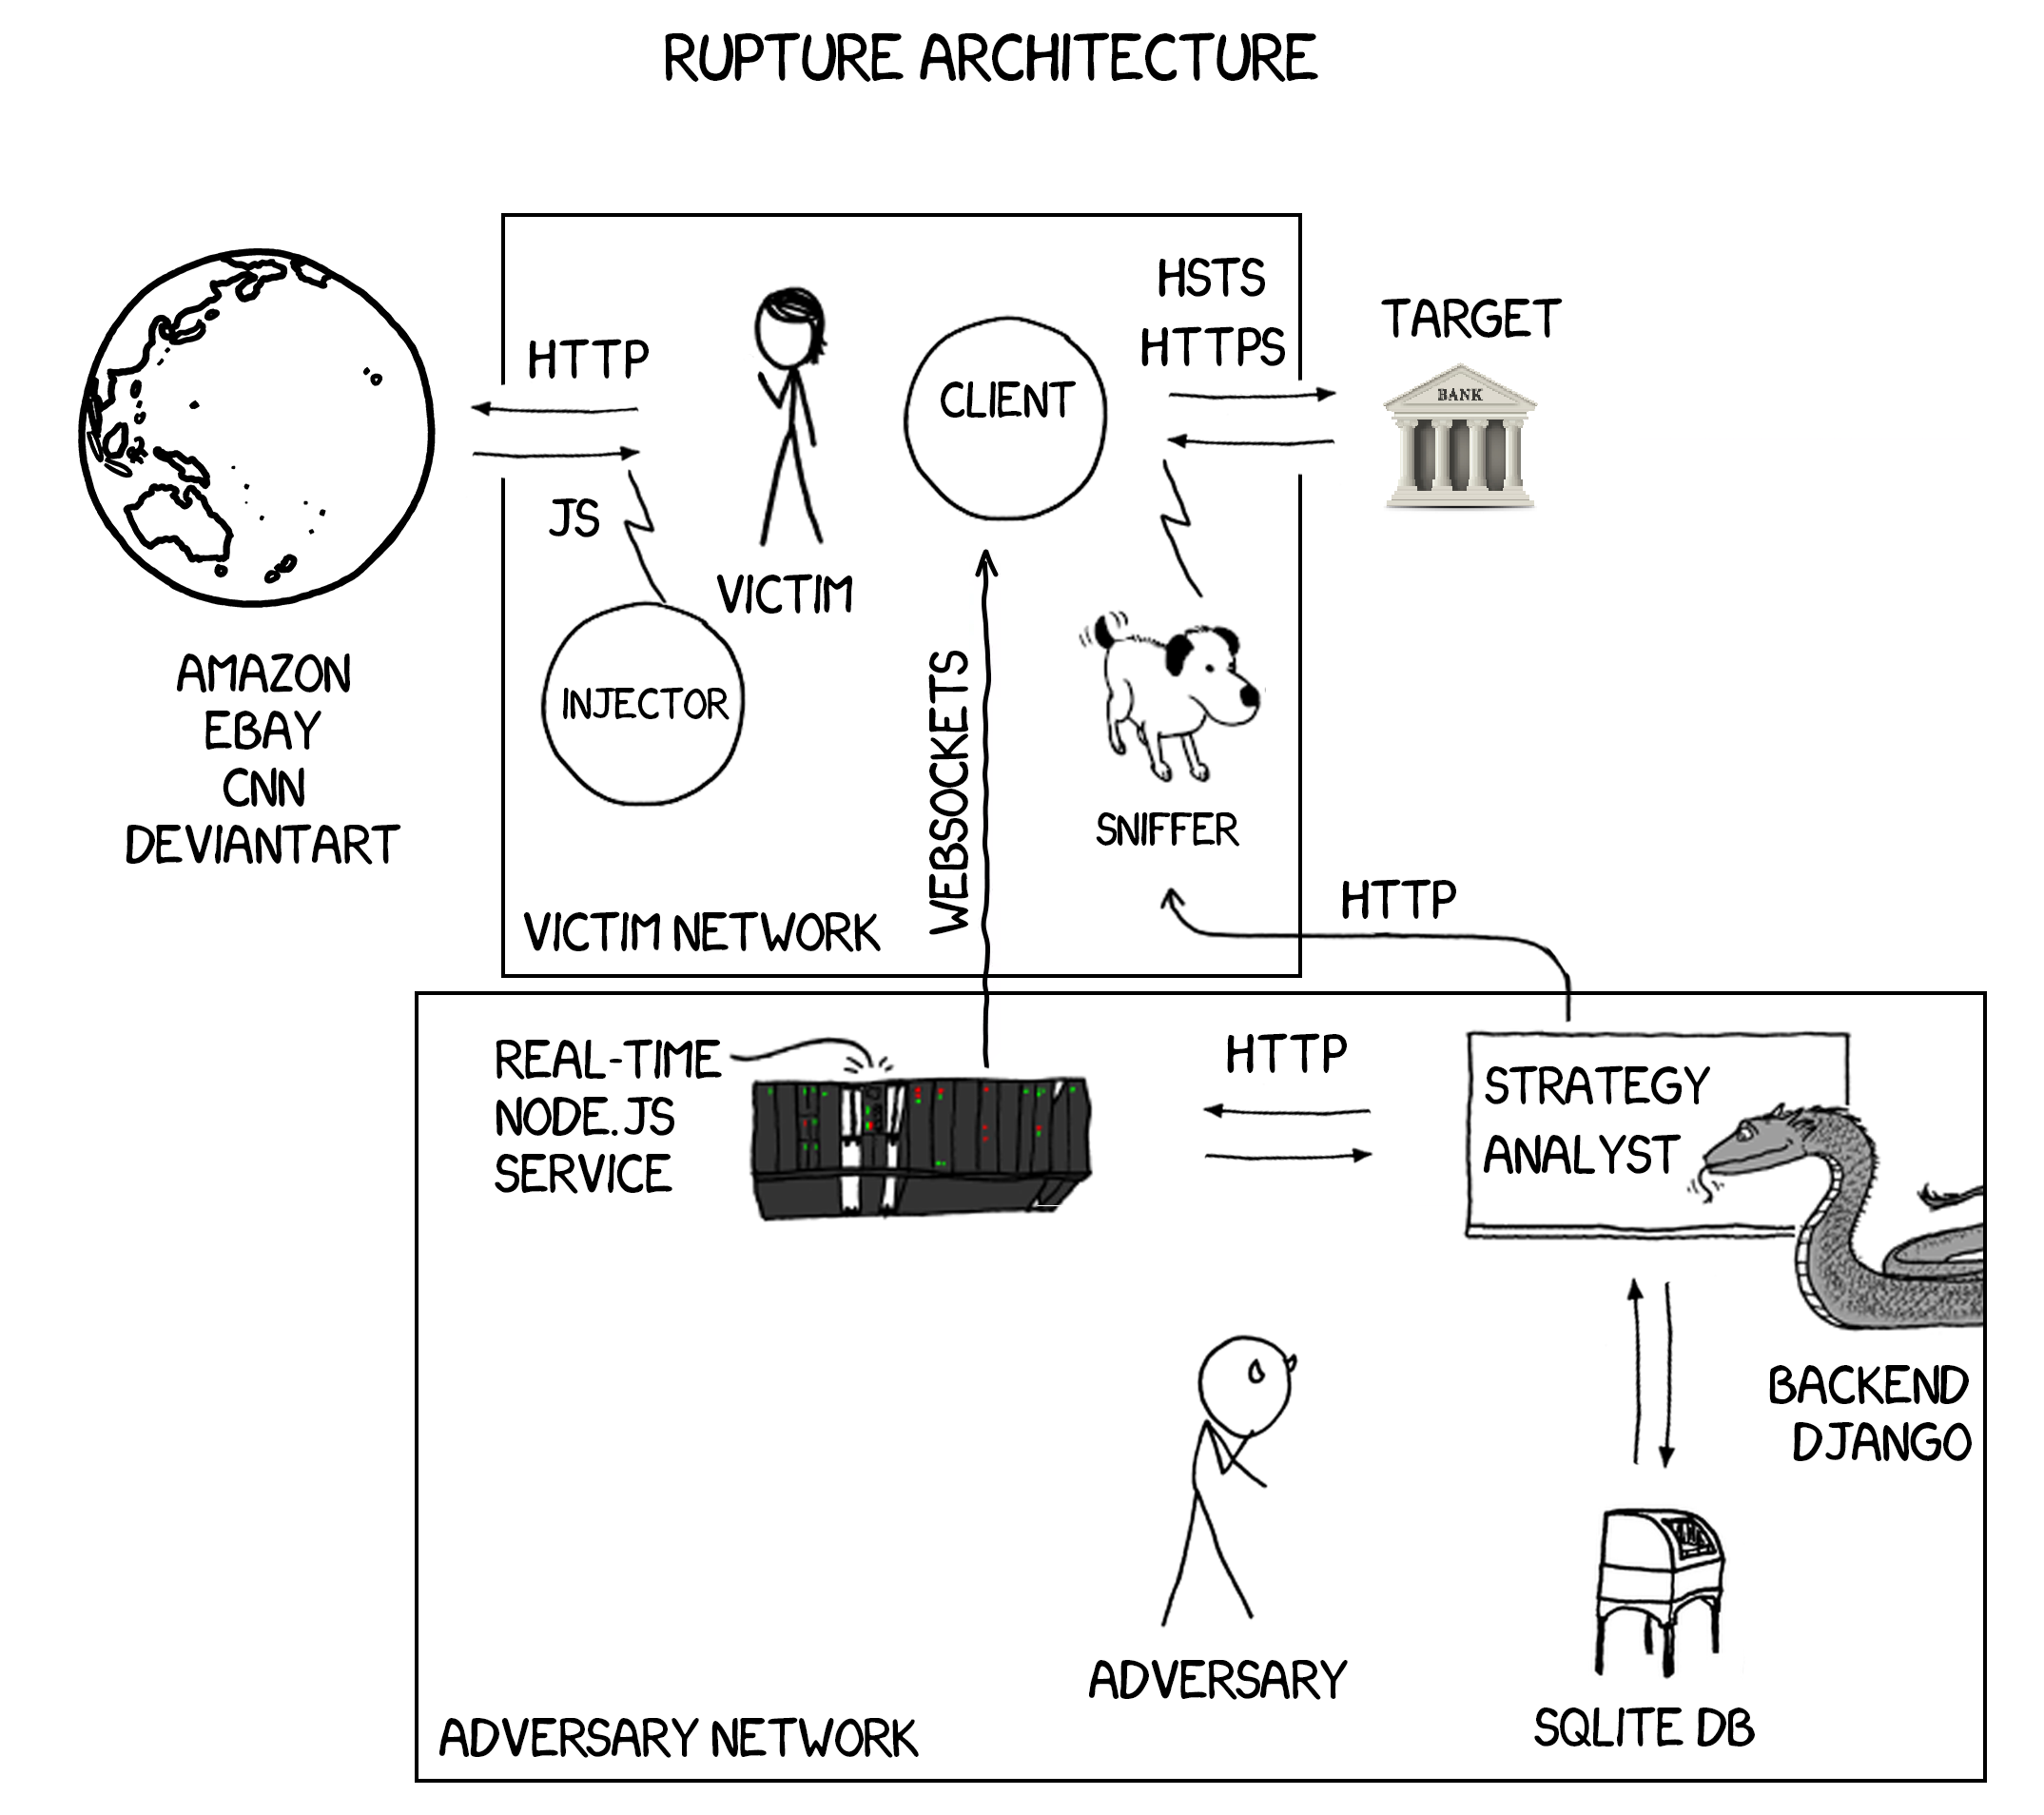
\includegraphics[width=0.48\textwidth]{figures/architecture.png}
      \caption{Rupture Architecture}
        \label{fig:rupture_architecture}
   \end{figure}

\subsubsection{Client}

The client component is a Javascript code that issues requests towards a chosen
endpoint. It needs to be executed from the browser of the victim, so that the
victim's authentication cookies are included in the request and the secrets are
included in the response. The client contains minimal logic by design. It
connects to the realtime service through a \textit{command-and-control} channel,
registers itself, and then waits for work instructions, which come in the form
of URLs for the requests it needs to make.

\subsubsection{Injector}

The injector component is responsible for injecting the client to the victim's
browser. The injection is performed by ARP spoofing (or NDP poisoning in the
case of IPv6) the local network and forwarding all traffic in a
Man-in-the-Middle manner. As the victim is browsing the Internet, multiple
clients will be injected in insecure pages and will run under various web contexts.
The fact that all HTTP responses are infected increases robustness,
as multiple injectors can be deployed to different networks, all controlled by the
same central command-and-control channel. The injector module is built using
Bettercap as the underlying tool for the network injection.

\subsubsection{Realtime}

The realtime is a service that acts as an intermediary between the clients and
the backend. When a client is injected in a page, it registers to the realtime and
maintains an open connection. Consequently the realtime holds command-and-control
connections with various clients which may live on different networks,
orchestrates them, and enforces the activation state for each one. It
activates one client per victim to receive work instructions and keeps the rest of
the victim's clients dormant. If the active client dies, for example by closing
its browser tab, one of the dormant clients is activated to continue the
attack. It also connects to the backend service using HTTP API calls to get
the work instructions for the active clients. The realtime is built in
Node.js \cite{tilkov2010node} and uses the socket.io framework
\cite{rai2013socket} for the command-and-control connections.

\subsubsection{Sniffer}

The sniffer component is responsible for collecting data from the victim's
network. When instructed, the sniffer collects the encrypted request and
response network packets for a given victim and a target. It also exposes a HTTP
API which is utilized by the backend for controlling when the sniffing starts and
stops, and to retrieve the sniffed data. It is built in Python, using Scapy
\cite{biondi2010scapy} for the network functionality.

\subsubsection{Backend}

The backend component is the center of operations for all attacks. It is
configured with the target and victim information, initializes the attacks and
designs the samplesets that should be collected.  When work needs to be done,
it forwards the instructions to the realtime in order to reach the clients. Meanwhile, it
orders the sniffer to listen for network traffic between the victim and the
target. When the client reports (via the realtime) that the work is completed, the
backend collects the traffic from the sniffer, analyzes the captured network
data and calculates the attack confidence for the round.
Therefore the backend is responsible for strategic decision taking and
adaptively advancing the attack. Based on statistical analysis of the network
samples, it decides if the collected samplesets are valid and if the confidence
is adequate for a round to be completed. It also stores persistent data about
the ongoing attack in a database for future analysis. It is built in Python,
using the Django framework for the RESTful API service.

\subsection{Optimizations}\label{subsec:optimizations}

Rupture incorporates a number of optimizations that allow for faster and more
robust execution of attacks against multiple protocols.

\subsubsection{Block alignment}\label{subsec:blockalign}
In block ciphers, the length of the encrypted text is rounded up to a product of
$\mu$-bits, where $\mu$ is the block size. Consequently, length difference
between two plaintexts does not always result in a similar length difference between the
respective ciphertexts.

We bypass this problem by using known block alignment techniques
\cite{moller2014poodle}. This method demands issuing multiple requests
and including artificial noise. In each request $r_{i, c_j}$
for each candidate $c_j$ in the alphabet, we add increasing artificial
noise of length $i$. That way, $r_{1, c_j}$ will contain one character of
alignment noise, $r_{2, c_j}$ two characters and so forth. Therefore, for some
alignment noise of length $a \in [0, \mu)$ the length of the request with the
correct candidate will be $(\delta*\mu)$ and for all incorrect candidates
$(\delta*\mu)+1$. In that case, the incorrect candidates result in one more
block compared to the correct one. This ensures that one out of $\ceil{\mu /
|r_i|}$ requests will result in a block distinction between the alphabet
candidates.

Figure \ref{fig:block_alignment} depicts the block alignment technique
intuitively.

   \begin{figure}[thpb]
      \centering
          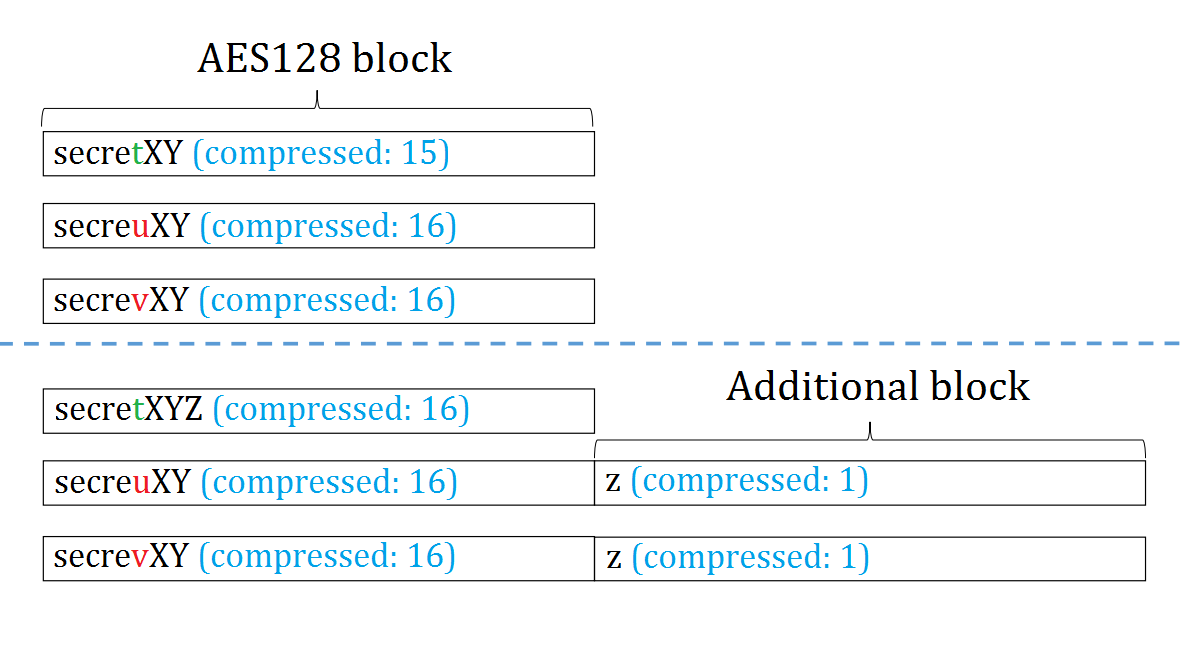
\includegraphics[width=0.48\textwidth]{figures/block_alignment.png}
      \caption{The block alignment method}
      \label{fig:block_alignment}
   \end{figure}

\subsubsection{Reflection computation methods}\label{subsec:reflectionmethods}
So far we have described the need for building and analysing reflections to
distinguish a single candidate in the secret's alphabet $\Sigma$ as the correct
one. In this section, we present two methods for constructing the reflections.

The first method is serial construction described in section
\ref{subsec:rupture_attack_design}. The complexity of this method is
$\mathcal{O}(|\Sigma|)$ and the round ends by finding a character of the secret.

The second method of attack is divide and conquer. The alphabet is now divided
into two subsets $\Sigma_1$ and $\Sigma_2 = \Sigma \setminus \Sigma_1$, where
$|\Sigma_1| = |\Sigma_2| = \ceil{|\Sigma| / 2}$. The reflection string for
$\Sigma_1$ consists of $|\Sigma_1|$ substrings separated by an annotation symbol
$\beta$. Each substring is built by concatenating the known prefix with a
candidate in $\Sigma_1$. For example, if $\Sigma_1$ is $\{``1", ``2"\}$ and the
known prefix is ``abc", using ``-" as $\beta$ the reflection is ``abc1-abc2".
The reflection string for $\Sigma_2$ is constructed similarly.

The end of each round marks the choice of subset $\Sigma_i$ that contains the
correct alphabet symbol. Each round reduces the alphabet by half, so the
complexity of this method is $\mathcal{O}(log|\Sigma|)$. When $|\Sigma_i| = 1$
the attack stage is completed and a character of the secret is decrypted.
Figure \ref{fig:divide_and_conquer} depicts the reflection sequence for the case
when the $\Sigma$ is the set of digits.

   \begin{figure}[thpb]
      \centering
          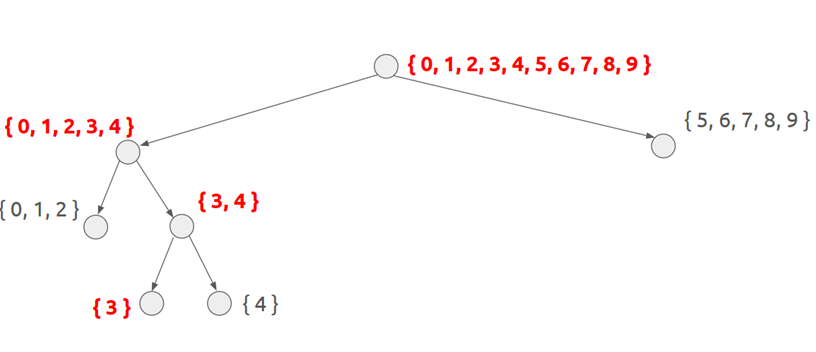
\includegraphics[width=0.48\textwidth]{figures/divide_and_conquer.png}
      \caption{The divide \& conquer method}
      \label{fig:divide_and_conquer}
   \end{figure}

\subsubsection{Request parallelization}\label{subsec:parallel}
Modern web servers are able to handle multiple parallel requests and
browsers can issue a certain amount of parallel requests per domain. This
functionality enables the adversary to issue multiple parallel requests per
candidate and efficiently reduce the execution time of the attack.

\subsubsection{Request soup}
Previous sections demonstrated the need for multiple requests per reflection
string $r_i$. However, communication is time expensive, so in many cases it is
preferable to issue multiple requests for a candidate and treat them as a set
rather than separately. This is the case for BREACH, where a set consists of
requests for a candidate $s_i$ in alphabet $\Sigma$. Bigger request sets result
in less time delay and the adversary can use the mean length over the number of
requests in the set without caring for each individual request's length.

\subsection{Experiments}\label{subsec:rupture_experiments}

In this section we provide results on various experiments we conducted in
laboratory environment to evaluate the performance of Rupture. These results
reflect Rupture's versatility when it comes to attacking different protocols and
are a good basis in order to evaluate the tool against real-world systems in
future work.

Our laboratory environment consisted of a single web page hosted on an
Nginx web server.\footnote[2]{The laboratory URLs used for experimentation have
been removed in the anonymized version of the paper.} This page contains digits
and a single secret word, which consists of 8 lowercase English letters.
The first two characters of the word are known and used
to bootstrap the attack. It also offers a GET URL parameter and reflects
the parameter's value among the digits in the page.

This page is the most basic scenario for a BREACH attack. It is noiseless and
the secret's alphabet is different from the rest of the page. We were also
careful to avoid the possibility of a wrong reflection compressing well with
parts of the page other than the secret.

We deployed all Rupture modules on a single machine and used this same machine
as the victim in order to avoid the need for injection. We also configured Rupture's
acceptable confidence level to 0.6 bytes and used the 26 lowercase English
letters as the secret's alphabet.

Finally, we utilized most optimizations proposed in the previous sections. We
used uppercase English letters for the block alignment, issued 32 requests
in parallel for each candidate in the form of a soup, and used the
divide and conquer method for computing the reflection strings.

Figure \ref{fig:rupture_performance_div_conq} shows the results of our first
experiment against the AES algorithm in GCM \cite{mcgrew2005galois} and CBC
modes for block sizes of 128 and 256 bits.

   \begin{figure}[thpb]
      \centering
          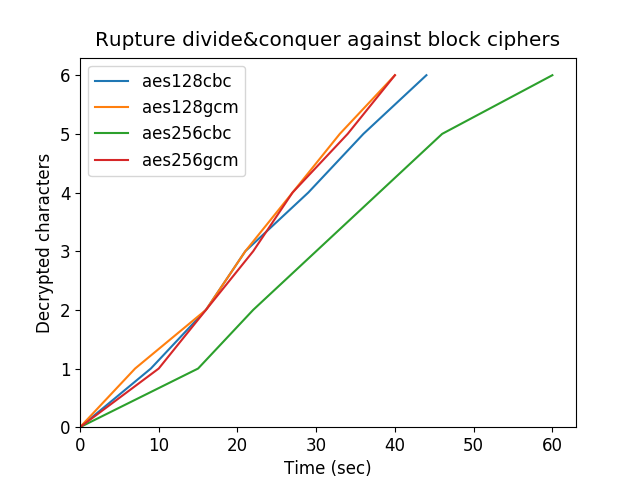
\includegraphics[width=0.48\textwidth]{experiments/rupture_performance/rupture_div_conq_performance.png}
       \caption{Rupture divide and conquer performance}
      \label{fig:rupture_performance_div_conq}
   \end{figure}

As can be seen, we were able to decrypt all 6 unknown characters of the word in
all cases. The total time for decrypting the characters ranged from 40 seconds,
in the case of GCM mode, to 60 seconds, in the case of CBC mode with 256-bit
block size. Therefore the average time for decrypting a single character using
the divide and conquer method was 6-10 seconds.

In our second experiment we tested the consistency of Rupture by targeting a
longer secret. This time the secret was 25 characters and we used the
serial method for computing the reflections. The rest of the experiment
parameters were the same as before. The results of this experiments are shown in
Figure \ref{fig:rupture_performance_serial}.

   \begin{figure}[thpb]
      \centering
          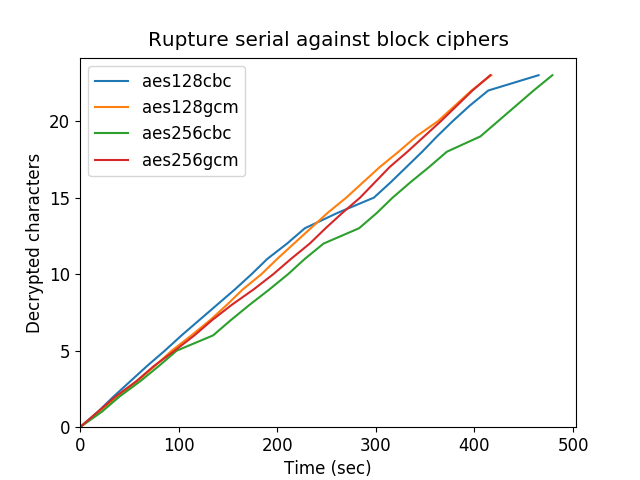
\includegraphics[width=0.48\textwidth]{experiments/rupture_performance/rupture_serial_performance.png}
      \caption{Rupture serial performance}
      \label{fig:rupture_performance_serial}
   \end{figure}

We were again able to decrypt all unknown characters in all AES modes and block
sizes. This time the total time ranged from 416 (GCM-256) to 479 (CBC-256)
seconds. Therefore the average time for decrypting a single character using the
serial method was 18-21 seconds.

We also notice that Rupture performs slightly worse against AES CBC compared to
AES GCM regardless of the block size. Further investigation on how different
modes affect the attack's performance should be conducted in future work.

\section{Reflection security}\label{sec:refsec}

We now define the theoretical model for reflection attacks. We propose a
cryptographic game for a simulation-based model and present proofs of insecurity
under the necessary assumptions. We then move on to describe the properties of
the various elements in the game and describe existing compression attacks,
including Rupture, as instances of the theoretical model we introduce.

\subsection{The reflection game}\label{subsec:refsecgame}

Let $\mathcal{T} = (Gen, K, \mathcal{D})$ be a triplet of algorithms. In this
triplet, $Gen$ is a key generation algorithm which, given a security parameter
$1^\lambda$ returns some key $\kappa$. The function $K$ is an encryption
function with three parameters: The key $\kappa$ and two plaintexts $s$ and $r$,
which we call the \textit{secret} and \textit{reflection} specifically. For now,
we leave the question of how these plaintexts are combined to be encrypted
together undefined; this will be instantiated into a concrete function when we
discuss the security of particular schemes.

Let $\mathcal{A}$ be an adversary and $\mathcal{S}$ be a simulator. Also let
$\mathcal{M}$ be a distribution of plaintexts and $g$ a function defined on its
support, as well as some function $Com(\cdot)$ defined on the domain of $K$. We
call $Com$ the compression function and require that it is a deterministic
polynomially computable and reversible bijection.

The game $\text{Game}_{\text{REF-SEC}}^{\mathcal{SE},\mathcal{A}}(\lambda)$ is
parameterized with the security parameter $\lambda$. The challenger produces a
$\lambda$-bit key $k \leftarrow Gen(1^\lambda)$ and initially
chooses a secret $s \leftarrow \mathcal{M}$.

The adversary is then allowed to run and make arbitrary calls to a reflection
oracle. The oracle is parameterized by $s$, the secret unknown to the adversary.
For the reflection oracle call, the adversary chooses a reflection string $r$
and sends it to the oracle. The oracle computes $c = K_\kappa(s, r)$.
Subsequently $c$ is sent back to the adversary.

When the adversary decides to complete the game, they output a guess $y$. The
adversary is successful if $g(s) = y$. In the case of Rupture, a successful
attack results in the decryption of a single character that extends the known
prefix of secret $s$.

Formally, let the secret key adversarial game be defined as follows:

\begin{lstlisting}[texcl,mathescape,basicstyle=\small]
def $\text{Game}_{\text{REF-SEC}}^{\mathcal{SE},\mathcal{A}}(\lambda)$:
    $k \leftarrow Gen(1^\lambda)$
    $s \leftarrow \mathcal{M}$
    $y \leftarrow \mathcal{A}^{\text{Reflect}^{k}_s(r)}(1^\lambda)$
    if $y = g(s)$:
        return 1
    else:
        return 0
\end{lstlisting}

Where the reflection oracle provided to the adversary is as follows:

\begin{lstlisting}[texcl,mathescape,basicstyle=\small]
def $\text{Reflect}^{k}_s(r)$:
    $c \leftarrow K_{k}(s, r)$
    return $c$
\end{lstlisting}

Let the simulator game be defined as follows:

\begin{lstlisting}[texcl,mathescape,basicstyle=\small]
def $\text{Game}_{\text{REF-SIM}}^{\mathcal{SE},\mathcal{S}}(\lambda)$:
    $s \leftarrow \mathcal{M}$
    $s' = 0^{|s|}$
    $y \leftarrow \mathcal{S}^{\text{Reflect}^{k}_{s'}(r)}(1^\lambda, {|Com(s)|})$
    if $y = g(s)$:
        return 1
    else:
        return 0
\end{lstlisting}

The reflection oracle provided to the simulator is as follows:

\begin{lstlisting}[texcl,mathescape,basicstyle=\small]
def $\text{Reflect}^{k}_{s'}(r)$:
    $c \leftarrow \mathcal{K}_{k}(s', r)$
    return $c$
\end{lstlisting}

Both the adversary and the simulator are given access to an encryption and decryption oracle, but
are not allowed to call the decryption oracle with the reflection oracle output.

The reflection game is depicted in Figure \ref{fig:refgame}.

    \begin{figure}[thpb]
        \centering
            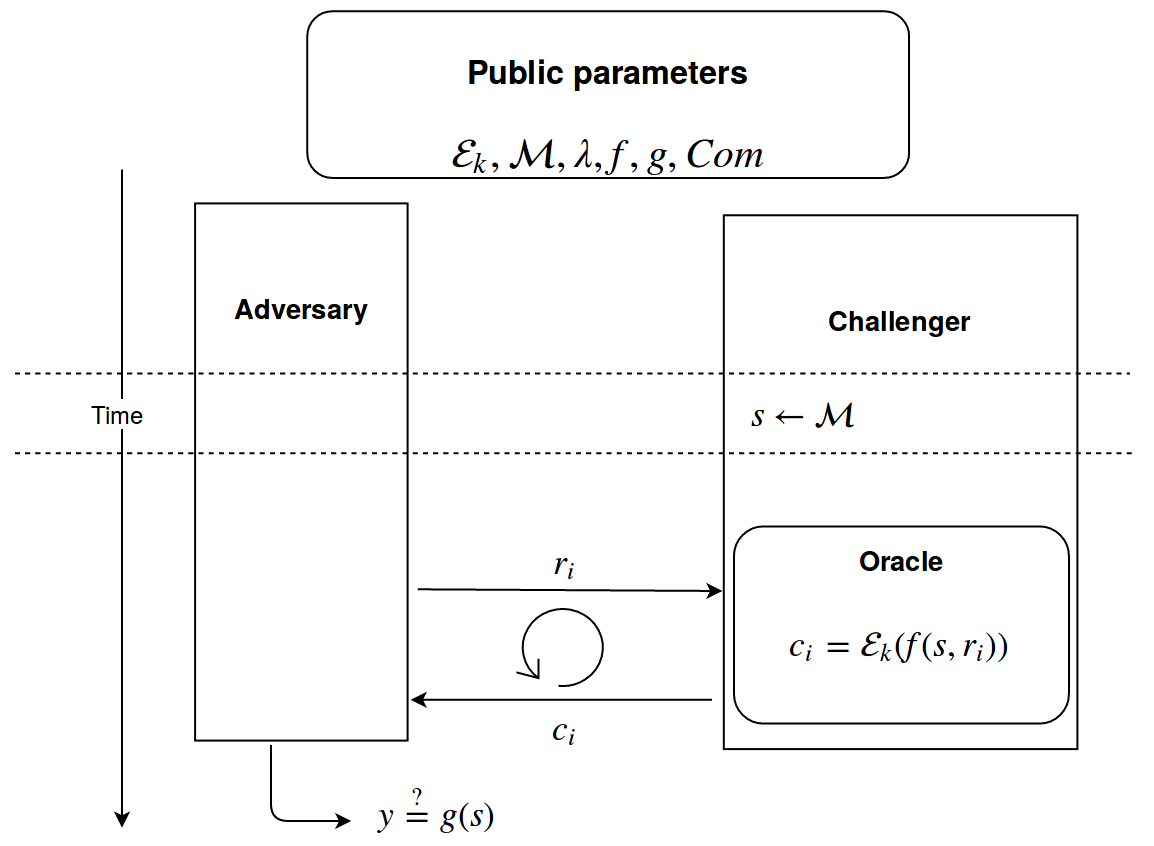
\includegraphics[width=0.48\textwidth]{figures/reflection_game.png}
        \caption{Reflection Game}
        \label{fig:refgame}
    \end{figure}

\subsection{Adversarial advantage}\label{subsec:refsecadv}

Let us now define the advantage of the adversary against a simulator:
\begin{align*}
    \text{Adv}_{\mathcal{SE}, \mathcal{A}, \mathcal{S}}&(\lambda) &\defeq\\
    |\Pr[\text{Game}_{\text{REF-SEC}}^{\mathcal{SE},\mathcal{A}}(\lambda) = 1] &-\\
    \Pr[\text{Game}_{\text{REF-SIM}}^{\mathcal{SE},\mathcal{S}}(\lambda) = 1]| &
\end{align*}

\subsection{Adaptive reflection security}\label{subsec:adaptiverefsec}

Given a rendering function $f(\cdot, \cdot)$, a private-key encryption scheme
$\mathcal{SE}$ composed with a rendering function $f$ is
\textit{reflection-secure} if:
\begin{align*}
    \forall \mathcal{M}:
    \forall g:
    \forall PPT \mathcal{A}:
    \exists PPT \mathcal{S}:\\
    \text{Adv}_{\mathcal{SE}, \mathcal{A}, \mathcal{S}}(\lambda) = negl(\lambda)
\end{align*}

\begin{lemma}[Semantic security]
    Let $(Gen, E, D)$ be a length-preserving reflection-secure encryption
    scheme. Then it is also semantically secure.
\end{lemma}

For a full proof, see Appendix A.

\subsection{The interdependence assumption}\label{subsec:interdependence}

Let $\bar{\mathcal{M}}$ be a joint distribution from which the random variables
$(s, r)$ are drawn. We say that $s$ and $r$ are interdependent when there exist
$s_1, r_1$ and $s_2, r_2$ in the support of $\bar{\mathcal{M}}$ with $s_1 \neq
s_2$ such that:
\begin{align*}
    \Pr[(s, r) = (s_1, r_1)] &< \Pr[(s, r) = (s_1, r_2)]
\land\\
    \Pr[(s, r) = (s_2, r_1)] &> \Pr[(s, r) = (s_2, r_2)]
\end{align*}

Where the pair $(s, r)$ is drawn from the joint distribution
$\bar{\mathcal{M}}$.

It is clear that when two random variables $s$ and $r$ exhibit interdependence,
they must necessarily be dependent random variables. To see that
interdependence is a stronger version of dependence, observe that in the case
of dependence, the probability for some $s = s_1$ conditioned on $r = r_1$ is
necessarily different from the probability for some $s = s_2$ conditioned on $r
= r_2$. In interdependence, it can be seen that we additionally require the
event $s = s_1$ which was less probable than the event $s = s_2$ under the
condition $r = r_1$ to become more probable than $s = s_2$ under the condition
$r = r_2$.

We observe that commonly compressed texts such as HTML content exhibit
interdependence almost everywhere. To be more precise, if we sample, for
example, digrams (two-letter sequences) in HTML content of popular websites and
treat this two-letter sequence $\phi = (s, r)$ of the two characters $s$ and $r$
as a random variable $\phi$, we notice that $s$ and $r$ are dependent variables
and in fact interdependent. This straightforward fact is supported by extensive
statistical analyses in the scientific literature such as
\cite{norvig2013english}.

While the interdependence assumption is a general notion observed in all common
plaintexts, it is suitable to mention here how these ideas will emerge as we
mount our attack. In a plaintext $(s, r)$ in which the attacker controls some
reflection string $r$ and wishes to obtain information about some secret string
$s$, she wishes to distinguish between the cases $s = s_1$ and $s = s_2$ of two
different secrets $s_1$ and $s_2$, i.e. between the instances $(s_1, r)$ and
$(s_2, r)$. By measuring the difference in the probability of $(s, r)$
occurring for $r = r_1$ and $r = r_2$, the attacker can distinguish which value
of $s$ is in use. If $s = s_1$, then the attacker will observe the inequality
$\Pr[(s, r) = (s_1, r_1)] < \Pr[(s, r) = (s_1, r_2)]$, but when $s = s_2$, the
attacker will observe the different inequality $\Pr[(s, r) = (s_2, r_1)] >
\Pr[(s, r) = (s_2, r_2)]$.

\subsection{Composing with compression}\label{subsec:comcompose}

We now shift our interest to algorithms which compose compression and
encryption. We define the composition of a compression algorithm with a
rendering function and an encryption algorithm.

The encryption scheme above is treated as a composition of a
compression and encryption algorithm:
\begin{equation*}
    \mathcal{E} = \textrm{Enc} \circ \textrm{Com}
\end{equation*}

$\textrm{Com}$ is any polynomially computable reversible function that takes an
input string and outputs a new string: $\textrm{Com}: \{0, 1\}^* \leftarrow \{0,
1\}^*$.

$\textrm{Enc}$ denotes an encryption function. We stress our important
assumption that $\textrm{Enc}$ is defined on $\{0, 1\}^*$ and not on some
fixed-length input.

Also, a text transformation function $\mathcal{K}$ is a function that has the
properties defined above and, for the rest of the paper, we treat it as a
compression function.

\subsection{Compression idealness}\label{subsec:com_idealness}

We now move on to define the notion of compression idealness.

Let $\mathcal{K}$ be a function defined on some domain and with output space
all strings $\{0, 1\}^*$, and let $\bar{\mathcal{M}}$ be a distribution whose
support is a subset of the domain of $\mathcal{K}$.  We say that $\mathcal{K}$
is an ideal compression function with respect to the distribution
$\bar{\mathcal{M}}$ when for every $w_1, w_2$ in the support of
$\bar{\mathcal{M}}$ we have:
\begin{equation*}
\Pr[w = w_1] < \Pr[w = w_2] \iff \lvert\mathcal{K}(w_1)\rvert > \lvert\mathcal{K}(w_2)\rvert
\end{equation*}

Where $w$ is a random variable drawn from $\bar{\mathcal{M}}$.

The intuitive notion behind compression idealness is that the encoding
function is somehow perfectly aware of the input distribution. It
exploits this knowledge of the input space to encode each possible
input in an ideal way - more often occurring plaintexts are compressed
better, i.e. in shorter length, than rarely occurring plaintexts.
Practical compression functions are not perfectly ideal, because the
distribution of plaintexts they try to cover is broad and ill-defined.
However, such compression functions try to learn the distribution of
the plaintext they are about to compress by observing frequencies of
occurrences and taking advantage of them.

We extensively investigate experimentally the idealness aspect of the LZ77 and
Huffman compression functions in Appendix \ref{subsec:idealness_experiment}.

\subsection{Length monotonicity}\label{subsec:lenmonotone}

An important assumption for our attack is that the encryption function
$\textrm{Enc}$ is \textit{length monotonic}. Specifically, for any keys $k_1,
k_2$ in the key generating function space and string messages $m_1, m_2$:
\begin{equation*}
\begin{split}
|m_2| > |m_1|
\Rightarrow
|\textrm{Enc}_{k_1}(m_2)| \geq |\textrm{Enc}_{k_2}(m_1)|
\end{split}
\end{equation*}

If the last inequality becomes strict, we call the encryption function
\textit{strictly length monotonic}.

A practical instance of a length monotonic encryption function is AES in GCM
mode. Stream ciphers can be treated as strictly monotonic to the bit level.

\subsection{Compressibility with respect to predicates}\label{subsec:propertycom}
In this section we will define compressibility with respect to predicates. We
show that all ideal compression functions that exhibit interdependence are
compression detectable by a reflection vector $\overbar{r}$ with respect to a
predicate $Q$ and a distribution $\mathcal{M}$.

Let $\mathcal{M}$ be a plaintext distribution and $Q(s)$ be a predicate on the
plaintext $s$ drawn from $\mathcal{M}$. Furthermore, we require that $Q$ is not a
trivial predicate; that is, there must exist elements for which $Q$ is true and
others for which it is false. Let us use $\mathcal{M}_Q$ to denote the
distribution $\mathcal{M}$ conditioned on the predicate $Q$.

For the specific property $Q$ and plaintext distribution $\mathcal{M}$, define:
\begin{equation*}
    \pi \defeq max(\Pr[Q(s)], 1 - \Pr[Q(s)])
\end{equation*}

Where $s$ is drawn from $\mathcal{M}$.

Let $\overbar{r} = (r_1, r_2) \in \mathcal{M}^2$ be a reflection string pair,
$\mathcal{K}$ be an ideal compression function, and let $\alpha(\lambda)$ be a
non-negligible function.

We now examine how the lengths of compressing a secret $s$ rendered with
reflection strings $r_1$ and $r_2$ respectively compare.

The predicate $Q$ partitions the set $\mathcal{M}$ into two partitions
$\mathcal{M}_Q$ and $\mathcal{M}_{\lnot Q}$. We are interested in reflection
string pairs $\overbar{r} = (r_1, r_2)$ for which the comparison direction
depends on which partition $s$ belongs to.  If $s \in \mathcal{M}_Q$, it should
compress better when reflection $r_1$ is used as compared to when $r_2$ is used.
On the contrary, if $s \in \mathcal{M}_{\lnot Q}$, the opposite direction should
occur.  If this is the case for the selected reflection pair, we say that $Q$
compares favourably under $\overbar{r}$:
\begin{equation*}
\begin{split}
    cpr^Q_{\mathcal{K}}(s, \overbar{r})
    \defeq\\
    \begin{cases}
        |\mathcal{K}(s, r_1)| < |\mathcal{K}(s, r_2)| &\text{ if } Q(s)\\
        |\mathcal{K}(s, r_1)| \geq |\mathcal{K}(s, r_2)| &\text{ otherwise}
    \end{cases}
\end{split}
\end{equation*}

The reflection pair $\overbar{r}$ \textit{detects} predicate $Q$ under
compression function $\mathcal{K}$ over the secret distribution $\mathcal{M}$ with
advantage $\alpha$ when the comparison is favourable for both $s_1$ drawn from
$\mathcal{M}_Q$ and $s_2$ drawn from $\mathcal{M}_{\lnot Q}$. Formally, we
define the predicate $dtc_\alpha(Q, \overbar{r}, \mathcal{K}, \mathcal{M})$
as follows:
\begin{align*}
    \Pr
        [cpr^Q_{\mathcal{K}}(s_1, \overbar{r}) \land
         cpr^Q_{\mathcal{K}}(s_2, \overbar{r})]
    \geq\\
    \pi + \alpha(\lambda)
\end{align*}

Where $s_1$ is drawn from $\mathcal{M}_Q$ and $s_2$ is drawn from
$\mathcal{M}_{\lnot Q}$.

We call $Q$ \textit{compression-detectable} with an advantage $\alpha$ if a pair
$\overbar{r} = (r_1, r_2)$ exists, such that $dtc_\alpha(Q, \overbar{r}, \mathcal{K},
\mathcal{M})$ holds. Furthermore we require that such a pair $\overbar{r}$ is
polynomially computable. That is, there exists some polynomial-time
functionality $\mathcal{O}_R(\mathcal{K}, Q, \mathcal{M})$ which produces an
$\overbar{r}$ such that $dtc_\alpha(Q, \overbar{r}, \mathcal{K}, \mathcal{M})$ holds.

The compression-detectability property exists in all common compression
functions as long as $s$ and $r$ compress in the same context. We will now
prove the fact that all compression functions which are ideal under some
distribution $\bar{\mathcal{M}}$ exhibit compression-detectability of some
predicate $Q$.

\subsection{Good compression allows predicate detection}

We now move on to show that all good compression functions exhibit
compression-detectability of some predicate. In intuitive terms, this means
that if a compression function compresses well enough, it will necessarily
allow one part of the plaintext to affect how another part of the plaintext
compresses. An attacker that is able to measure how well a string compresses
can use this to detect a predicate on the second part of the plaintext by
changing the first part of the plaintext.

In the following theorem, we prove compression detectability of a predicate with
the simplification that the resulting reflection pair $(r_1, r_2)$ is
efficiently computable.


\begin{lemma}[Good compression is detectable]
Let $\mathcal{K}$ be an ideal compression function with respect to some
interdependent distribution $\bar{\mathcal{M}}$. Then there exists
some compression-detectable predicate $Q$ for $\mathcal{K}$.
\end{lemma}

A full proof can be found on Appendix A.

\subsection{One-shot attack}

\begin{lemma}[Compression attack]

Let $\textrm{Com}$ be a compression function, $\textrm{Enc}$ be a strictly length-monotonic
encryption function, $f$ be a rendering function and $Q$ be a plaintext
predicate detectable with non-negligible advantage $\alpha$ over plaintext
distribution $\mathcal{M}$.

Then:
\begin{align*}
    \exists \alpha \text{ non-negl}:
    \forall \textrm{Enc}:
    \exists g:\\
    \exists PPT \mathcal{A}:
    \forall PPT \mathcal{S}:\\
    \text{Adv}_{\mathcal{SE}(\textrm{Enc}, \textrm{Com}), \mathcal{A}, \mathcal{S}}
    (\lambda, f, \mathcal{M}, g) = \alpha(\lambda)
\end{align*}

\end{lemma}

For a full proof, see Appendix A.

\subsection{Amplified attack}\label{subsec:amplification}

We can now amplify the attack to achieve a better probability of success by a small modification in our adversary.
The amplification is parameterized by an odd parameter $k$.

Let the amplification adversary be defined as follows:

\begin{lstlisting}[texcl,mathescape,basicstyle=\small]
def $\mathcal{A}(Q, \mathcal{M})$:
    $(r_1, r_2) \leftarrow \mathcal{O}_R(\textrm{Com}, f, Q, \mathcal{M})$

    $low = 0$
    $high = 0$

    for $i$ = $0$ to $k$:
        $l_1 = |\text{Reflect}^{\mathcal{E}_{pk}}_s(r_1)|$
        $l_2 = |\text{Reflect}^{\mathcal{E}_{pk}}_s(r_2)|$

        if $l_1 < l_2$:
            $low = low + 1$
        else:
            $high = high + 1$

    if $low > high$:
        return True
    else:
        return False
\end{lstlisting}

\begin{lemma}[Amplification]

Under the assumptions of the Compression Attack Theorem against $f, \textrm{Com}$
and compression-detectable predicate $Q$ with non-negligible
detectability margin $\alpha(\lambda)$,
the amplified adversary achieves an arbitrarily large advantage
against a non-negligible subset of elements, the
\textit{amplifiable elements} distinguished by predicate $Amp$.
\begin{align*}
    \forall \textrm{Enc}:
    \exists g:\\
    \exists PPT \mathcal{A}:
    \forall PPT \mathcal{S}:\\
    \exists Amp:
    \exists B \text{ non-negl}:
    \exists C \text{ negl}:\\
    \Pr_{s \leftarrow \mathcal{M}}[Amp(s)] = B(\lambda) \land\\
    \text{Adv}_{\mathcal{SE}(\textrm{Enc}, \textrm{Com}), \mathcal{A}, \mathcal{S}_{Amp}}
    (\lambda, f, \mathcal{M}, g) = 1 - \pi - C(k)
\end{align*}

\end{lemma}

The complete proof can be found in Appendix A.

\section{Defending against compression attacks}\label{sec:defense}
Keeping in mind our theoretical model, we determine the key elements that make these
attacks possible.

We propose a defense, \textit{context hiding}, that mitigates a class of
practical compression side-channel attacks such as CRIME, TIME, BREACH, Rupture,
and HEIST. The full plaintext recovery these attacks perform is no longer
possible when our defense is applied.

\subsection{Hardness of defending}
First of all, observe that there is a trivial method of defense, and that is
disabling compression completely.

However, defending against an adversary by modifying $f$ is hard in general. We
note that $f$ is required to be polynomially reversible, meaning it must contain
enough information to recover $s$. Because $Com$ must be able to decrease the
length of various plaintexts, it can output plaintexts of different lengths
dependent on $s$. Therefore, if $Com$ is adversarial, it can easily leak
information through the encryption function $Enc$ by using its output length. As
such, any attempt to generally defend against all compression functions $Com$ is
necessarily futile.

However, the fact that it is theoretically difficult to define a generic defense
should not discourage us from pursuing a practical defense that applies in
practice along with the specific compression functions currently in use. In
this direction, we give a series of arguments based on our previously developed
theory for why we believe our defense method is secure.

\subsection{Attack elements from a defense perspective}
The basic problem that needs to be solved is the compression detectability of the
predicate $Q$ under this class of attacks. In order to eliminate detectability,
it should be made impossible for any pair of reflections $\overbar{r}$ to detect
$Q$ under the compression function $\textrm{Com}$ and the rendering function
$f$. In order to achieve this there exist two options - either change the
compression or the rendering function.

The next step is determining what kind of changes are needed. We therefore
consider the notions that make detectability possible. These notions are
compression idealness and interdependence. The first is part of the composition
of $\textrm{Com}$ and $f$, whereas the second is part of $f$. That said, removing
either of these notions from the functions will strip the adversary of the ability
to detect $Q$.

The first choice is forcing the compression function to act non-ideally in the
cases of secrets. Proposed defenses like disabling compression for annotated
secrets are based on this exact idea. However, as we will see when experimentally
evaluating our proposed defense, this option might add considerable performance
overhead.

The second choice is removing the interdependence between reflections and
secrets. In order to achieve that we need to decorrelate the probability of
secrets and reflections. One way to achieve this is by encrypting the secret.
Another method that acts similarly is secret masking, described in section
\ref{subsec:masking}.

Context hiding builds on the latter option while achieving very good balance on
performance cost and security.

\subsection{Context hiding properties}

Context hiding is built on the premise of separating secrets in a per-origin
manner in order to avoid cross-compression. In order to achieve this we define
what constitutes an origin and what properties same-origin secrets share.

\subsubsection{Origin}
An origin is a uniquely identifiable party that generates content. A party can
be either a physical entity, like a user, or an application. It is important to
properly identify the party that generated a piece of content, as the definition
of origins reflects the amount of knowledge over same-origin content.
However, the CTX origin should not be confused with the origin definition in the
same-origin policy \cite{ruderman2001same}. The CTX origin is not bounded by the
restrictions of the same-origin policy and reflects a more intuitive notion on who
generated a piece of content and what knowledge he has over the rest of the
content.

\subsubsection{Same-origin secrets}
After assigning origins, we consider each piece of content a secret. It is
implied that all secrets that have been assigned the same origin should have
been generated by the party that this origin identifies. An immediate result of
this assumption is that anyone with access to a secret $s$ of origin $o$ also
has access to all other secrets $s'$ of the same origin $o$.

\subsection{Context hiding functionality}
Our defense method disables cross-compression by applying a simple substitution
cipher derived from a random permutation of the origin's alphabet.

Firstly, we identify the origins of the plaintext $m$ and store them in the
array $origins$. Each secret $s_i$ in $m$ is identified by its origin. Each
origin is uniquely identified by an integer in range $[0, |origins|)$.

Secondly, we identify the alphabet for each origin. An origin's alphabet is the
set of characters of all secrets identified by this origin. For each origin, we
generate a random permutation of the origin's alphabet and store it in the array
$permutations$. The first element in the $permutations$ array corresponds to the
first origin in the $origins$ array and so forth.

In order to secure a secret $s$ we apply the hiding function \textit{hide}. This
function takes two arguments, the secret $s$ and the permutation $p$ of the
secret's origin, applies the substitution cipher on each character in $s$ and
returns the permuted secret $s'$.

\begin{lstlisting}[texcl,mathescape,basicstyle=\small]
def hide($s, p$):
    $s' = ''$
    for $c \in s$:
        $s' = s' || Permute_p(c)$
    return $s'$
\end{lstlisting}

The function $Permute_p(c)$ implements the substitution cipher. It finds the
index $i$ in the origin's alphabet for the character $c$ and returns the $i$-th
character in the permutation $p$.

The protected secret $s'$ is annotated by the special characters
$\beta_{start}^i$ and $\beta_{end}^i$, that mark the beginning and the end of any
substring that needs to be unpermuted and are unique per origin. The output $m'$
that is produced after hiding all secrets consists of all permuted texts
concatenated with the permutation array $permutations$.

The initial secret $s$ can be retrieved from the protected secret $s'$ using the
\textit{unhide} function. This function takes $s'$ and permutation $p$ of the
secret's origin and applies the reverse permutation on $s'$.

\begin{lstlisting}[texcl,mathescape,basicstyle=\small]
def unhide($s', p$):
    $s = ''$
    for $ch \in s'$:
        $s = s || Permute_p^{-1}(ch)$
    return $s$
\end{lstlisting}

In our theoretical model, we assume that there exists a single secret. However,
in this section we generalize this and we treat the reflection $r$ and the
secret $s$ as two secrets of different origins. The fact that
$s$ and $r$ are permuted with different permutations for each call to the oracle
makes it impossible for an adversary controlling $r$ to learn
information about $s$, as he would have to decrypt the entire plaintext using
only a single request.

\section{CTX: Mitigating BREACH with Context Hiding }\label{sec:ctx}

Our contributions include a defense framework which is implemented in the
application layer and is opt-in. We choose to update the rendering function $f$
instead of the compression function $\textrm{Com}$ as it requires less effort
from an engineering perspective. Our proposal requires no changes in the
underlying compression algorithms in the web server, such as Apache's
mod\_deflate. Instead, it only requires modifications in the web application
layer and can be easily incorporated in existing applications.

\subsection{Implementation}
CTX is an implementation of the context hiding method described in the previous
section, which secures web applications and HTML web pages.

When setting up the defense, it is the application developer's responsibility to
decide which portions of the response are sensitive and must be protected as
secrets. Sensitive data does not only include high-value secrets such as
passwords and CSRF tokens, but also any data that the developer wishes to keep
private. Some examples are the bodies of email messages, chat messages, or the
contents of documents and spreadsheets. In principle any piece of information
which is only accessible when logged in is a secret and should be CTX protected.

The amount of origins can range between one origin for the entire response and one
origin per character. The former would not CTX-protect any part of the
plaintext, while the latter would result in the best possible security under
CTX, although compression would be effectively disabled.

Secrets are permuted by the server using the generated permutation for their origin,
so different-origin secrets are forced to compress separately, i.e. not
cross-compress. However, same-origin secrets form a context and are compressed
together.

The response is then encrypted, sent over the network and, upon arrival on the
client side, the inverse permutation is applied to decode each secret. The
default alphabet for the origins is ASCII characters (0 - 128), which is randomly
permuted using the Fisher-Yates shuffle algorithm \cite{fisher1938statistical}.

Each time the server issues an HTTPS response, new per-origin permutations are
generated. However, compression side-channel attacks rely on the assumption that we can
perform multiple requests to the target website while the transmitted secret
remains the same. Since new alphabet permutations are generated per HTTPS
response, the statistical analysis performed by Rupture is no longer feasible.

\subsection{Experiments}\label{subsec:ctx_experiments}

We have conducted several experiments to evaluate the performance of web
services protected by CTX. The results of these experiments are overwhelmingly
positive.

The CTX parameters that affect performance are: the number of origins, the total
response size in bytes, and the amount of secrets in the response. Each
parameter affects the performance differently and will be examined thoroughly
below. Our experiments focused on each parameter separately, so the results
reflect the performance under each one independently.

In our tests we use an HTML web page where the secrets are strings of English
literature. The tests measure the performance penalty in terms of size overhead
in the compressed response HTML and time overhead, in the cases when it is more than 10ms.

However, it should be noted that our tests are particularly strict. A typical
website response consists mainly of HTML code or libraries that usually need not
be protected. In this case, the amount of secrets in the response would not
exceed 1\% of the total response, in which case the CTX overhead observed during
our experiments is realistically acceptable. For example, Facebook and Gmail,
which offer web pages that are ~600KB would typically need only protect approximately
0.5\% of the response.

The first parameter, the number of origins, mainly affects the compression
performance of the secrets. More origins result in larger response, both
compressed and uncompressed. This is expected, given the fact that secrets from
different origins do not cross-compress.

Our experiment covered a 650KB web page, which consists of 1\% secrets and 99\%
static data. The secrets are evenly distributed in origins that range from 1 to
50. Since the total amount of secrets and static data is independent to the
number of origins, the length of all same-origin secrets is reduced as the
number of origins increases. We consider 50 origins a reasonable choice, since a
typical response nowadays contains data generated by multiple users and
services.

    \begin{figure}[thpb]
        \centering
            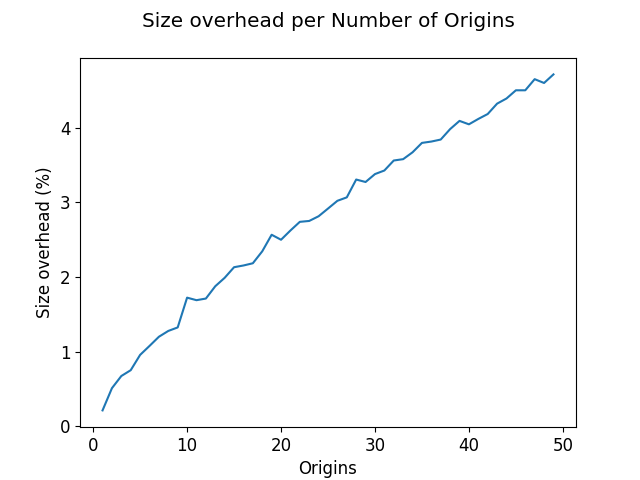
\includegraphics[width=0.48\textwidth]{experiments/ctx_performance/origins.png}
        \caption{Origins}
        \label{fig:origin_ctx}
    \end{figure}

As Figure \ref{fig:origin_ctx} shows, the size overhead when 1 origin is used is
less than 0.5\% and about 4.7\% when 50 origins are used. This means that in our
worst-case scenario, the compressed CTX-protected response is 1.047 times the
unprotected compressed response.

The second parameter, the total response size, reflects the scalability of CTX.
In this case, we use 50 origins and consider 1\% of the total response to be
secret, equally distributed in all origins. The length of the response page
ranges from 13KB to 650KB.

Our experiments show that the increase in bytes that CTX adds is not
proportional to the increase of the total response size. This results in a
significant overhead for small web pages, which becomes less observable as the
web page grows larger.

    \begin{figure}[thpb]
        \centering
            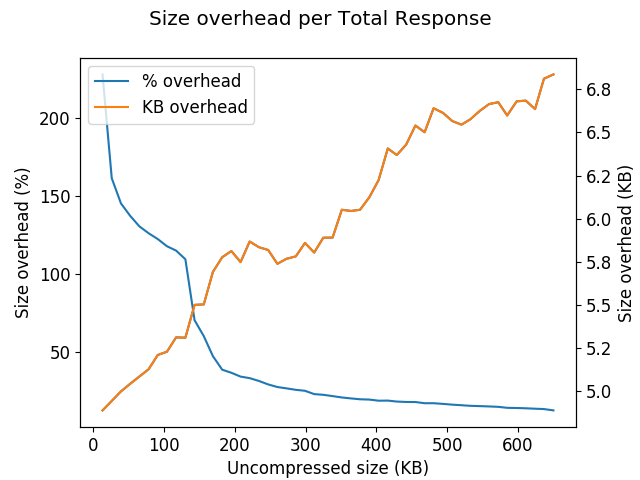
\includegraphics[width=0.48\textwidth]{experiments/ctx_performance/total_response.png}
        \caption{Total response}
        \label{fig:total_response_ctx}
    \end{figure}

Figure \ref{fig:total_response_ctx} depicts the results of this experiment. A
13KB web page suffers a 5KB CTX overhead, which corresponds to a 228\% increase
in compressed response. On the other hand, CTX will add only 7KB for a 650KB web
page, which results in a 12\% increase. In comparison, the overhead for
disabling compression entirely would range from 500\% to 1000\% for the tested
web pages, while, for this last case of the 650KB web page, the secret masking
method previously suggested in the literature adds a 21\% overhead.

The third parameter is the total amount of secrets in the response. We now use
a 650KB web page with 50 origins. The secrets amount from 1\% up to 50\% of the
web page, the rest being static data, and are evenly distributed across origins.

    \begin{figure}[thpb]
        \centering
            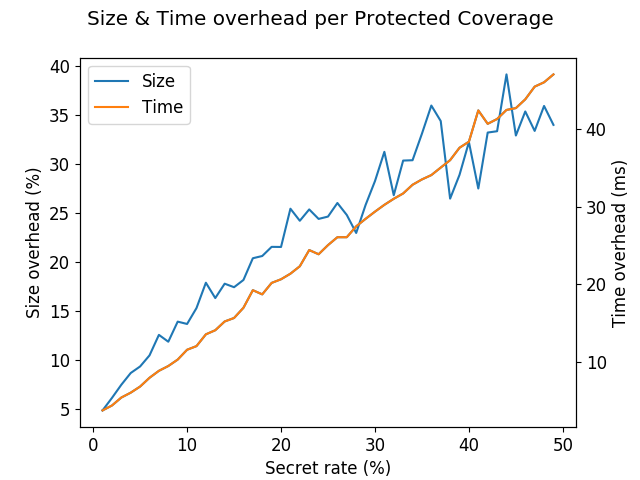
\includegraphics[width=0.48\textwidth]{experiments/ctx_performance/response_secrets.png}
        \caption{Response secrets}
        \label{fig:response_secrets_ctx}
    \end{figure}

Figure \ref{fig:response_secrets_ctx} shows the results of this experiment. We
find that protecting 1\% of this web page results in less than 5\% size
overhead, whereas protecting 50\% of the page results in 35\% overhead. The time
increase is also noteworthy in this case, where CTX adds 10ms of execution time
for 10\% secrets in the web page and 47ms for 50\% secrets.

In comparison, disabling compression would result in 976.8\% load overhead
and a network transmission time overhead that, depending on the client's and the
server's network, may be several seconds.

\subsection{Security of CTX}

We now move on to describe a series of lemmas that show certain conditions
which allow for provable reflection security. This direction supports
the design decisions for CTX. While we do not formally prove the security of
CTX, we argue that it is empirically similar to provably secure schemes.

We start by providing the full proof for a simple construction. We then move on
to provide proof sketches for consecutively more complicated constructions,
until we reach a construction which we argue is very similar to CTX.

In the lemmas below, we use the shorthand $E$ to refer to the encryption
function of an encryption schema $(Gen, E, D)$. We talk about the reflection
security of various schemes which are defined by their output. For example,
when we say that $E(s) || E(r)$ is reflection secure, we mean that the function
defined as $\widetilde{E}(s, r) = E(s) || E(r)$ is reflection secure.

Complete proofs of all lemmas can be found in Appendix A.

\begin{lemma}[Reflection-independent security]
    Let $E$ be a length-preserving semantically secure encryption schema and
    $Com$ be any function. Then $E(s)$ is reflection secure.
\end{lemma}

\begin{lemma}
    Under the above assumptions, $E(s) || r$ is reflection secure.
\end{lemma}

\begin{lemma}
    Under the above assumptions and letting $Com$ be a deterministic
    efficiently computable function, $E(s)$ $||$ $Com(r)$ is reflection secure.
\end{lemma}

\begin{lemma}
    Under the above assumptions and additionally requiring that $Com$ is a
    bijection which is also efficiently reversible, $E(Com(s))$ is reflection secure.
\end{lemma}

\begin{lemma}
    Under the above assumptions, $E(Com(s)) || r)$, \break$E(Com(s)) || E(r))$, and
    $E(Com(s)) || E(Com(r))$ are all reflection secure.
\end{lemma}

\begin{lemma}
    Under the above assumptions, $E(s || r)$ is reflection secure.
\end{lemma}

\begin{lemma}
    Under the above assumptions, $E(Com(s)$ $||$ $Com(r))$ is reflection secure.
\end{lemma}

We are now ready to argue for the security of CTX. Let the function $ctx(s)$
denote the substitution cipher applied on $s$ using a uniformly random alphabet
permutation. We make the simplifying assumption that $ctx(s)$ only contains the
ciphertext where the substitution cipher has been applied and that the exact
permutation required to reverse the substitution cipher is sent through a
separate secure channel.

Under the assumption that \[|Com(s) || Com(r)| = |Com(ctx(s) || ctx(r))|\] we
see that the semantically secure function $E$ will not allow distinguishing
between the two distributions $Com(s) || Com(r)$ and $Com(ctx(s) || ctx(r))$.

Clearly, these two lengths will not be equal for adversarial compression
functions Com. However, we argue that they are almost equal for realistic
instances of compression functions.

In order to back our claim, we perform the following experiment. We choose a
fixed secret $s$, 100 characters long. We then choose the reflections $r_i,
i\in[0, 50]$, where $|r_i| = 50 + i*20$. For each $r_i$ we calculate the
length of separate compression using gzip $|gzip(s)||gzip(r_i)|$ and the length
of the compressed CTX'ed secret and reflection $|gzip(ctx(s), ctx(r_i))|$, where $s$
and $r_i$ belong to different origins.

The results are shown in figure \ref{fig:defense_experiment}. It can be seen
that the outputs of these two methods are linearly correlated, with the
Pearson correlation coefficient of the two variables being 0.998712.

    \begin{figure}[thpb]
        \centering
            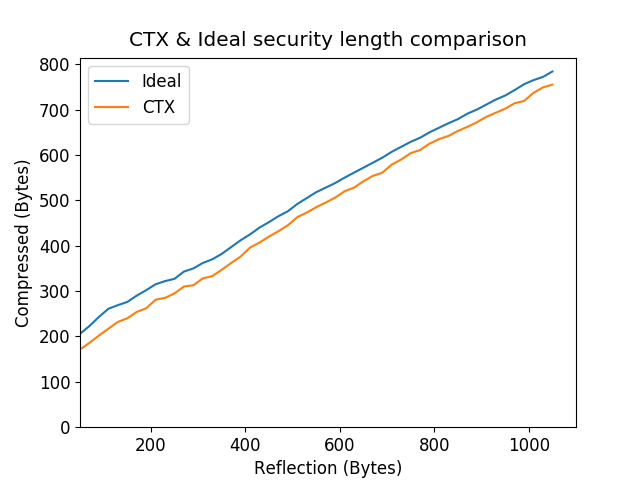
\includegraphics[width=0.48\textwidth]{experiments/ctx_idealness/ctx_experiment.png}
        \caption{CTX/Theoretical security comparison}
        \label{fig:defense_experiment}
    \end{figure}

\section{Related work}\label{sec:related}

\subsection{Compression attacks}

The compression side-channel attack technique was first studied by Kelsey
\cite{kelsey2002compression} in 2002. Kelley and Tamassia\cite{kelley2014secure}
discuss the notion of \textit{entropy-restricted} semantic security. However,
this only models the case where two secrets compress to the same length, making
it difficult to capture practical techniques used in attacks such as BREACH.

Alawatugoda et al. \cite{alawatugoda2015protecting} introduce a model for \textit{Cookie recovery},
\textit{Random cookie indistinguishability}, and \textit{Chosen cookie indistinguishability}.
Nevertheless, their security models are limited to classes of rendering functions
that are very specific. In their models, the attacker is able to directly influence
the output of the rendering function through concatenation.

\subsection{Defenses}

\subsubsection{Disabling compression}\label{subsec:disablecom}
Compression is the basic assumption for the compression detectability, so disabling
compression would break the adaptive reflection game. However, this is not a
viable solution. Disabling compression results in a performance penalty that
outweighs the benefits of the defense.

\subsubsection{SameSite cookies}\label{subsec:samesite}
SameSite cookies \cite{mwest2015firstparty} is a proposed draft for enhancing
web security. The main puprose of this technique is to mitigate cross-site
request forgery attacks. It introduces a new attribute for web cookies, that web
servers may opt-in, which states that cookies may only be included in a
``first-party" context, i.e. in same origin requests. The current BREACH
application depends on cross-origin requests in order to call the reflection
oracle, so enabling SameSite cookies would result in the elimination of this
type of reflection oracle of the Reflection-Security Game.

\subsubsection{Masking secrets}\label{subsec:masking}
Masking is a method for hiding a secret's properties. A mask is a random
bitstream in the secret's size, which is XORed with the secret and concatenated
with the masked output. The secret can then be obtained by applying XOR between
the masked secret and the mask. This method doubles the size of the protected
secret, while also weakening the compression performance. Therefore, it is
applied on high value secrets only, in order to avoid significant performance
penalties. It is used by Facebook \cite{facebookbreach} in order to protect CSRF
tokens against BREACH attacks.

\section{Future work}

Rupture demonstrated very positive results against block ciphers in a basic
scenario. The next step is investigating its performance against noisy endpoints
and real-world systems, bypassing issues of compression with irrelevant content
pieces, and testing different AES modes and other encryption algorithms. There
is also a need for a formal proof of CTX's security based on the given lemmas.


\bibliographystyle{ACM-Reference-Format}
\bibliography{citations}

\appendix
\section{Full proofs}

\begin{lemma}[Semantic security]
\end{lemma}

\begin{proof}
    We will prove that if the scheme is not semantically secure, then it is
    necessarily not reflection secure. Assume that the scheme is not
    semantically secure. Then there will exist a PPT adversary $\mathcal{A}$
    such that for all PPT simulators $\mathcal{S}$ we have that $\mathcal{A}$
    has non-negligible advantage to $\mathcal{S}$ in the semantic security game.

    We will now construct an adversary $\mathcal{A'}$ for the reflection
    security game. $\mathcal{A'}$ operates as follows: It makes one query to
    the reflection oracle setting $r_0 = \epsilon$ and receives a response $c_0
    = K_k(s, r_0) = K_k(s) = c$. It then passes that $c$ to the semantic
    security adversary $\mathcal{A}$. It answers all encryption and decryption
    queries of the semantic security adversary by relaying them to its own
    encryption and decryption oracle. Finally, when the semantic security
    adversary outputs $y = y'$, this $y'$ is output by the reflection security
    adversary. Note that $\mathcal{A}$ cannot distinguish whether they are
    playing against the actual semantic security game or being simulated by the
    reflection security adversary, as their view is identical. Therefore:

    \begin{equation}
        Pr[Game_{REF-SEC}^{\mathcal{A'}} = 1] = Pr[Game_{SEM-SEC}^{\mathcal{A}} = 1]
    \end{equation}

    It remains to prove that $\mathcal{A'}$ has significant advantage against
    any reflection simulator $\mathcal{S'}$. Indeed let $\mathcal{S'}$ be any
    reflection game simulator. We will construct a simulator $\mathcal{S}$ for
    the semantic security game. Initially, the simulator $\mathcal{S}$ receives
    the length of the ciphertext $|c|$. They then simulate the reflection game
    simulator $\mathcal{S'}$ as follows. Upon receiving query $r_i$ from the
    reflection game simulator, they answer with $|c| + |r_i|$. When the
    reflection security adversary outputs $y' = y$, this $y$ is output by the
    semantic security simulator. We observe that the reflection game simulator
    $\mathcal{S'}$ cannot distinguish whether they are playing against the
    actual simulated reflection game or being simulated by the semantic
    security simulator. To see this, note that from the length preservation
    assumption we have that $|c| + |r_i| = |K(s, r_i)| = |K(s', r_i)| =
    |K(0^{|s|}, r_i)|$. Therefore:

    \begin{equation}
        Pr[Game_{SEM-SIM}^{\mathcal{S}} = 1] = Pr[Game_{REF-SIM}^{\mathcal{S'}} = 1]
    \end{equation}

    From the assumption that the scheme is not semantically insecure, we know
    that:

    \begin{align*}
        |Pr[Game_{SEM-SEC}^{\mathcal{A}} = 1] - Pr[Game_{SEM-SIM}^{\mathcal{S}} = 1]| =\\
        Adv_{\mathcal{A}, \mathcal{S}} = \text{non-negl}
    \end{align*}

    And therefore, replacing both probabilities with their equals:

    \begin{align*}
        |Pr[Game_{REF-SEC}^{\mathcal{A'}} = 1] -
        Pr[Game_{REF-SIM}^{\mathcal{S'}} = 1]| =\\
        Adv_{\mathcal{A'}, \mathcal{S'}} = \text{non-negl}
    \end{align*}
\end{proof}

\begin{lemma}[Good compression is detectable]
\end{lemma}

\begin{proof}
We model our plaintext input to the compression function as the usual pair $(s,
r)$ consisting of the secret string $s$ and reflection string $r$. When $(s, r)$
are encoded by a compression function $\mathcal{K}$ ideal under some plaintext
distribution $\bar{\mathcal{M}}$, a simple predicate allows the distinction
between two secrets $s_1$ and $s_2$ using a reflection pair $(r_1, r_2)$.  We
make the assumption that the resulting reflection pair $(r_1, r_2)$ is
efficiently computable.

\begin{align*}
    \Pr[r = r_1|s = s_1] < \Pr[r = r_2|s = s_1]&\land\\
    \Pr[r = r_1|s = s_2] > \Pr[r = r_2|s = s_2]&
\end{align*}

Using the fact that $\mathcal{K}$ is ideal with respect to this distribution,
we deduce that:

\begin{align*}
    |\mathcal{K}(s_1, r_1)| > |\mathcal{K}(s_1, r_2)|&\land\\
    |\mathcal{K}(s_2, r_1)| < |\mathcal{K}(s_2, r_2)|&
\end{align*}

We then define $Q(s)$ to be the predicate ``$s = s_1$". This partitions
$\mathcal{M}$ into the distributions $\mathcal{M}_Q$ and
$\mathcal{M}_{\lnot Q}$ both of which are non-empty, as $\mathcal{M}_Q$
contains $s_1$ and $\mathcal{M}_{\lnot Q}$ contains $s_2$. From the fact that
$Q$ is not trivial, we deduce that $\pi < 1$.

Observe, then, that letting $\bar{r} = (r_1, r_2)$ we obtain:

\begin{align*}
    \Pr[cpr^Q_{\mathcal{K}}(s_1, \bar{r}, \mathcal{K}, \mathcal{M})
    \land
    cpr^Q_{\mathcal{K}}(s_2, \bar{r}, \mathcal{K}, \mathcal{M})] = 1
\end{align*}

This completes the proof.

\end{proof}

\begin{lemma}[Compression attack]
\end{lemma}

\begin{proof}

Let $g$ be the boolean function $Q$ on the plaintext. Define the adversary
$\mathcal{A}$ as follows:

\begin{lstlisting}[texcl,mathescape,basicstyle=\small]
def $\mathcal{A}(1^\lambda)$:
    $(r_1, r_2) \leftarrow \mathcal{O}_R(1^\lambda)$

    $l_1 = |\text{Reflect}^{k}_s(r_1)|$
    $l_2 = |\text{Reflect}^{k}_s(r_2)|$

    if $l_1 < l_2$:
        return True
    else:
        return False
\end{lstlisting}

Let $\mathcal{S}$ be an arbitrary simulator. Then we have:
\begin{align*}
    \Pr[\text{Game}_{\text{REF-SIM}}^{\mathcal{SE},\mathcal{S}}
        (\lambda) = 1] &=\\
    \Pr_{x \leftarrow \mathcal{M}, b \leftarrow \mathcal{S}(1^\lambda)}
        [Q(x) = b]
\end{align*}

Letting the random variables $b$ and $x$:
\begin{align*}
    x &\leftarrow \mathcal{M}\\
    b &\leftarrow \mathcal{S}(1^\lambda)
\end{align*}

Due to the independence of the simulator's output with the choice of $x$ we have:
\begin{align*}
    Pr[b = Q(x)] &=\\
    Pr[\lnot b|\lnot Q(x)]Pr[\lnot Q(x)] + Pr[b|Q(x)]Pr[Q(x)] &=\\
    Pr[\lnot b]Pr[\lnot Q(x)] + Pr[b]Pr[Q(x)] &=\\
    (1 - Pr[b])(1 - Pr[Q]) + Pr[b]Pr[Q(x)] &=\\
    1 - Pr[Q(x)] - Pr[b] + 2Pr[b]Pr[Q(x)]
\end{align*}

For a given $\Pr[Q]$, this function is monotonic in $\Pr[b]$ and therefore has
potential extrema at $\Pr[b] = 0$ or $\Pr[b] = 1$, for which cases the function
takes the values $1 - \Pr[Q(x)]$ and $\Pr[Q(x)]$ respectively. Therefore, the
maximum $\Pr[b]$ of the simulator is:
\begin{equation*}
    \Pr[Q(x) = b] = max(\Pr[Q(x)], 1 - \Pr[Q(x)]) = \pi
\end{equation*}

And therefore:
\begin{align*}
    \forall \mathcal{S}:\\
    \Pr[
        \text{Game}_{\text{REF-SIM}}^{\mathcal{SE},\mathcal{S}}
        (\lambda) = 1
    ]
    \leq\\
    max(Pr[Q(x)], 1 - Pr[Q(x)])
\end{align*}

From the compression detectability of Q we know that:
\begin{align*}
    \exists \alpha \text{ non-negl}:\\
    \Pr_{s_1 \leftarrow \mathcal{M}_Q,
         s_2 \leftarrow \mathcal{M}_{\lnot Q}}
         [cpr^Q_{\kappa}(s_1, \overbar{r}) \land
          cpr^Q_{\kappa}(s_2, \overbar{r})]
    \geq\\
    \pi + \alpha(\lambda)
\end{align*}

Therefore:
\begin{align*}
    \Pr_{s_1 \leftarrow \mathcal{M}_Q}
         [cpr^Q_{\kappa}(s_1, \overbar{r})]
    \geq
    \pi + \alpha(\lambda) \land\\
    \Pr_{s_2 \leftarrow \mathcal{M}_{\lnot Q}}
         [cpr^Q_{\kappa}(s_2, \overbar{r})]
    \geq
    \pi + \alpha(\lambda)
\end{align*}

And so:
\begin{align*}
    \Pr_{s \leftarrow \mathcal{M}}
         [cpr^Q_{\kappa}(s, \overbar{r})]
    =\\
    \Pr[cpr^Q_{\kappa}(s, \overbar{r})|Q(s)]\Pr[Q(s)]
    +\\
    \Pr[cpr^Q_{\kappa}(s, \overbar{r})|\lnot Q(s)]\Pr[\lnot Q(s)]
    \geq\\
    (\pi + \alpha(\lambda))(\Pr[Q(s)] + (1 - \Pr[Q(s)))
    =\\
    \pi + \alpha(\lambda)
\end{align*}

Let us now examine the event of $\mathcal{A}$ being successful, denoted Succ,
when $cpr^Q_{\kappa}(s, \overbar{r})$. Assuming $Q(s)$:
\begin{align*}
    \Pr[|\mathcal{K}(s, r_1)| < |\mathcal{K}(s, r_2)||Q(s)]
    = \pi + \alpha(\lambda)
\end{align*}

And from the strict length monotonicity of $\textrm{Enc}$ it follows that:
\begin{align*}
    \Pr[&|\textrm{Enc}(\mathcal{K}(s, r_1))| <\\&|\textrm{Enc}(\mathcal{K}(s, r_2))||Q(s)]
        \geq \pi + \alpha(\lambda)\\
    \Rightarrow \Pr[&
        |\text{Reflect}^{k}_s(r_1)|
        <
        |\text{Reflect}^{k}_s(r_2)||Q(s)
    ]
        \geq \pi + \alpha(\lambda)\\
    \Rightarrow \Pr[&l_1 < l_2|Q(s)]
        \geq \pi + \alpha(\lambda)\\
    \Rightarrow \Pr[&\text{Succ}|Q(s)]
        \geq \pi + \alpha(\lambda)\\
\end{align*}

The case for $\lnot Q(s)$ is the same, but with a different inequality direction:
\begin{align*}
    \Pr[|\mathcal{K}(s, r_1)| > |\mathcal{K}(s, r_2)||\lnot Q(s)]
        \geq\\
        \pi + \alpha(\lambda)\\
    \Rightarrow \Pr[\text{Succ}|\lnot Q(s)] \geq\\
    \pi + \alpha(\lambda)\\
\end{align*}

And so the probability of success is given:
\begin{align*}
    \Pr[\text{Succ}] =\\
    \Pr[\text{Succ}|Q(s)]\Pr[Q(s)]
    +
    \Pr[\text{Succ}|\lnot Q(s)]\Pr[\lnot Q(s)] \geq\\
    \pi + \alpha(\lambda)
\end{align*}

Therefore,
\begin{align*}
    \forall PPT \mathcal{S}:
    \text{Adv}_{\mathcal{SE}(\textrm{Enc}, \textrm{Com}), \mathcal{A}, \mathcal{S}}
        (1^\lambda)
    \geq\\
    |\pi + \alpha(\lambda) - \pi| = \alpha(\lambda)
\end{align*}

Which is non-negligible.

\end{proof}

\begin{lemma}[Amplification]
\end{lemma}

\begin{proof}

From the fact that $Q$ is compression-detectable and from the Compression Attack Theorem, we have that:
\begin{align*}
    \Pr_{s \leftarrow \mathcal{M}}
         [cpr^Q_{\kappa}(s, \overbar{r})]
    =\\
    \pi + \alpha(\lambda)
\end{align*}

Some elements $s \in \mathcal{M}$ allow for better compression detectability than others under the fixed
reflection vector $\overbar{r}$. Call these elements \textit{amplifiable} and define predicate:
\begin{align*}
    Amp(s) \defeq
    \Pr[cpr^Q_{\kappa}
     (s, \overbar{r})]
    \geq
    \frac{1}{2} + \frac{\alpha(\lambda)}{2}
\end{align*}

We will now obtain a lower bound on the probability of an element being amplifiable.

Let:

% B derivation: (where \beta(\lambda) = \alpha(\lambda) / 2)
% B + (\frac{1}{2} + \alpha(\lambda)/2)(1 - B) = \pi + \alpha(\lambda)
% B + \frac{1}{2} + \alpha(\lambda)/2 - B(\frac{1}{2} + \beta(\lambda)) = \pi + \alpha(\lambda)
% \frac{1}{2} + \beta(\lambda) + B(\frac{1}{2} - \beta(\lambda)) = \pi + \alpha(\lambda)
% B(\frac{1}{2} - \beta(\lambda)) = \pi + \alpha(\lambda) - \frac{1}{2} - \beta(\lambda)
% B = (\pi + \alpha(\lambda) - \frac{1}{2} - \beta(\lambda)) / (\frac{1}{2} - \beta(\lambda))
% B = (\pi + \alpha(\lambda) - \frac{1}{2} - \frac{\alpha(\lambda)}{2}) / (\frac{1}{2} - \frac{\alpha(\lambda)}{2})
% B = (\pi - \frac{1}{2} + \frac{\alpha(\lambda)}{2}) / (\frac{1}{2} - \frac{\alpha(\lambda)}{2})
% B = \pi / (\frac{1}{2} - \frac{\alpha(\lambda)}{2}) - (\frac{1}{2} - \frac{\alpha(\lambda)}{2}) / (\frac{1}{2} - \frac{\alpha(\lambda)}{2})
% B = \pi / (\frac{1}{2} - \frac{\alpha(\lambda)}{2}) - 1
\begin{align*}
    B = \frac{\pi}{\frac{1}{2} - \frac{\alpha(\lambda)}{2}} - 1
\end{align*}

$B$ is non-negligible in $\lambda$.

Assume, for the sake of contradiction, that:
\begin{align*}
    \Pr_{s \leftarrow \mathcal{M}}
    [Amp(s)] < B
\end{align*}

Then we have:
\begin{align*}
    \Pr_{s \leftarrow \mathcal{M}}
         [cpr^Q_{\kappa}(s, \overbar{r})]
    =\\
    \Pr_{s \leftarrow \mathcal{M}}
         [cpr^Q_{\kappa}(s, \overbar{r})|Amp(s)]\Pr[Amp(s)]
    +\\
    \Pr_{s \leftarrow \mathcal{M}}
         [cpr^Q_{\kappa}(s, \overbar{r})|\lnot Amp(s)]\Pr[\lnot Amp(s)]
    <\\
    B + (\frac{1}{2} + \frac{\alpha}{2})(1 - B)
\end{align*}

But then:
\begin{align*}
    B + (\frac{1}{2} + \frac{\alpha(\lambda)}{2})(1 - B) =
    \pi + \alpha(\lambda)
\end{align*}

And this contradicts the assumption that $Q$ is compression-detectable. Therefore:
\begin{align*}
    \Pr_{s \leftarrow \mathcal{M}}
    [Amp(s)] \geq B
\end{align*}

It remains to show that the advantage of the adversary can be
arbitrarily large, i.e. that for some negligible $C$ we have:
\begin{align*}
    \text{Adv}_{\mathcal{SE}(\textrm{Enc}, \textrm{Com}), \mathcal{A}, \mathcal{S}_{Amp}}
    (1^\lambda) = 1 - \pi - C
\end{align*}

Indeed, observe that the amplifying adversary performs a repeated Bernoulli
trial with $k$ repetitions and extracts a majority. Let $X$ be the number of
repetitions that are successful for the adversary. $X$ is defined:
\begin{align*}
    X \defeq |\{ i: cpr^Q_{\kappa}(s, \overbar{r}) \}|
\end{align*}

$X$ follows the binomial distribution, and therefore its expected value is:
\begin{align*}
    E[X] = \frac{k}{2} + \frac{\alpha k}{2}
\end{align*}

Let Succ denote the event of the amplified adversary succeeding. Then Succ
is equivalent to $X > \frac{k}{2}$.

Because $\alpha$ is non-negligible and due to the tail bounds of the binomial
distribution, we have:
\begin{align*}
    Pr[Succ] = 1 - C(k)
\end{align*}

Where $C$ is a negligible function.
\end{proof}

\begin{lemma}[Reflection-independent security]
    Let $E$ be a length-preserving semantically secure encryption schema and
    $Com$ be any function. Then $E(s)$ is reflection secure.
\end{lemma}

\begin{proof}
    Let $\mathcal{A}$ be a reflection security adversary for $E(s)$. We will
    construct a semantic security adversary $\mathcal{A'}$ for $E$. Our semantic
    security adversary will break semantic security for \textit{multiple
    messages}. Let $\mathcal{M}$ be the distribution that $\mathcal{A}$
    attacks. Because $\mathcal{A}$ is a probabilistic polynomial-time
    adversary, there is a polynomial bound $t(\lambda)$ for its execution time.
    The number of reflection queries conducted by $\mathcal{A}$ is then also
    bound by $t(\lambda)$.

    Define $\mathcal{M'}$ by the following procedure: First, $s$ is chosen
    out of the distribution $\mathcal{M}$. Then that same $s$ is repeated
    $t(\lambda)$ times to obtain the vector of plaintexts $\overbar{s}$.

    Upon execution, $\mathcal{A'}$ receives from its challenger the encrypted
    vector $\overbar{c}$ where the same plaintext has been independently
    encrypted $t(\lambda)$ times.
    $\mathcal{A'}$ answers encryption and decryption queries of $\mathcal{A}$
    by forwarding them to its own encryption and
    decryption oracles. For reflection queries, because the schema trivially
    ignores $r$ since $E(s)$ is independent of $r$, the semantic security
    adversary is able to answer each query $r_i$ with $c_i$.

    Clearly, the view of the simulated reflection adversary is the same as if
    it were run in an actual reflection game. Therefore we have:

    \begin{align*}
        Pr[\text{Game}_{\text{REF-SEC}}^{\mathcal{A}}(1^{\lambda})
        = 1]
        =
        Pr[\text{Game}_{\text{SEM-SEC}}^{\mathcal{A'}}(1^{\lambda})
        = 1]
    \end{align*}

    We now prove that the adversary $\mathcal{A'}$ obtains a non-negligible gap
    against any semantic security simulator $\mathcal{S'}$. Indeed let
    $\mathcal{S'}$ be any semantic security simulator. We will construct a
    reflection security simulator $\mathcal{S}$. $\mathcal{S}$ works as
    follows: It obtains $|Com(s)|$ from its challenger which it ignores. It
    then issues a single reflection query $r_1 = \epsilon$, to which the
    challenger responds with $c = E(s')$. But $|c| = |E(s')| = |s'| =
    |0^{|s|}| = |s| = |E(s)| = |c|$ due to length preservation. This $|c|$ is
    then used to start the semantic security simulator.

    The view of the simulated semantic simulator is the same as if it were run
    in an actual semantic simulation game. Therefore we have:

    \begin{align*}
        Pr[\text{Game}_{\text{REF-SIM}}^{\mathcal{S}}(1^{\lambda})
        = 1]
        =
        Pr[\text{Game}_{\text{SEM-SIM}}^{\mathcal{S'}}(1^{\lambda})
        = 1]
    \end{align*}

    Because there exists a non-negligible advantage between $\mathcal{A}$ and
    any simulator $\mathcal{S}$, this gap will also exist between the
    constructed simulator $\mathcal{S}$. Therefore, we have:

    \begin{align*}
        \text{non-negl} = \text{Adv}_{\text{REF} \mathcal{A}, \mathcal{S}}\\
        =
        Pr[\text{Game}_{\text{REF-SEC}}^{\mathcal{A}}
        = 1] -
        Pr[\text{Game}_{\text{REF-SIM}}^{\mathcal{S}}
        = 1]\\
        =
        Pr[\text{Game}_{\text{SEM-SEC}}^{\mathcal{A'}}
        = 1]
        -
        Pr[\text{Game}_{\text{SEM-SIM}}^{\mathcal{S'}}
        = 1]\\
        =
        \text{Adv}_{\text{SEM} \mathcal{A'}, \mathcal{S'}}
    \end{align*}

    For clarity, we have omitted the security parameters from the games.
    This completes the proof.
\end{proof}

\begin{lemma}
    Under the above assumptions, $E(s) || r$ is reflection secure.
\end{lemma}

\begin{proof}
    The construction is identical to the previous proof. However, the
    reflection queries of the reflection adversary $\mathcal{A}$ must be
    answered correctly. As $r_i$ is known to the semantic security adversary,
    this can be done in the obvious way by setting $c_i' = c_i || r_i$.

    The reflection security simulator is not affected, as it receives $|c| =
    |Enc(s) || \epsilon| = |Enc(s)|$.
\end{proof}

\begin{lemma}
    Under the above assumptions and letting $Com$ be a deterministic
    efficiently computable function, $E(s)$ $||$ $Com(r)$ is reflection secure.
\end{lemma}

\begin{proof}
    The construction is the same as before. Because the semantic security
    adversary has access to the $Com$ function, it can calculcate $Com(r_i)$
    upon receiving the query $r_i$. Then setting $c_i = E(s) || Com(r_i)$ it
    responds as usual.

    The reflection simulator on the other hand will be affected by this
    construction. Indeed $|c| = |E(s') || Com(\epsilon)|$. However,
    $|Com(\epsilon)|$ can be computed by the simulator, and therefore the value
    given to the semantic simulator can be obtained as $|c'| = |E(s)| = |E(s')|
    = |c| - |Com(\epsilon)|$.
\end{proof}

\begin{lemma}
    Under the above assumptions and additionally requiring that $Com$ is a
    bijection which is also efficiently reversible, $E(Com(s))$ is reflection secure.
\end{lemma}

\begin{proof}
    This construction is slightly more complicated. Assuming $\mathcal{A}$ is a
    reflection-security adversary which works against the distribution
    $\mathcal{M}$ we will construct a multiple messages semantic security
    adversary as before. However, the distribution $\mathcal{M'}$ will now be
    obtained by the following procedure: Initially, $s$ is chosen out of
    $\mathcal{M}$. Then $Com(s)$ is calculated. This value is then repeated
    $t(\lambda)$ times. Our semantic security adversary will work against
    $\mathcal{M'}$.

    When the challenger produces the encrypted vector $\overbar{c}$, it will
    contain $t(\lambda)$ encryptions of the plaintext $Com(s)$. These can
    readily now be passed to the reflection adversary as reflection query
    responses as before.

    The reflection security simulator now makes use of the $|Com(s)|$ input,
    which it uses to start up the semantic security simulator.

    We now argue that the advantage obtained pertains to a valid predicate on
    the compressed plaintexts space. Indeed, without loss of generality assume
    that $g$ is a predicate. Then $g$ partitions the plaintext space into two
    partitions. Due to $Com$ being a bijection, these partitions are preserved
    after compression and the plaintext predicate $g$ is isomorphic to a
    compressed text predicate $g'$. Therefore, the semantic security adversary
    is able to obtain a non-negligible advantage for a different predicate.
\end{proof}

\begin{lemma}
    Under the above assumptions, $E(Com(s)) || r)$, \break$E(Com(s)) || E(r))$, and
    $E(Com(s)) || E(Com(r))$ are all reflection secure.
\end{lemma}

\begin{proof}
    The proofs for the above schemas can be combined in the obvious way to
    obtain the result needed.
\end{proof}

\begin{lemma}
    Under the above assumptions, $E(s || r)$ is reflection secure.
\end{lemma}

\begin{proof}
    We provide a sketch of this proof.

    To obtain this proof, we construct a semantic security adversary which
    works against a distribution $\mathcal{M'}$ defined as follows. First, $s$
    is chosen out of $\mathcal{M}$. Because the reflection security adversary
    is bounded in time by $t(\lambda)$, therefore each of the reflection
    queries $r_i$ must be $|r_i| < t(\lambda)$. The distribution $\mathcal{M'}$
    then will contain $t(\lambda)$ different vectors, each of dimension
    $t(\lambda)$. We require that the $j$-th $t$-dimensional vector contains
    the same secret text $s$ and an independently chosen reflection text $r$
    with $|r| = j$.

    Then the semantic security adversary $\mathcal{A'}$ works as follows: Upon
    receiving the reflection query $r_i$ from the reflection adversary, it
    responds with a fresh element from the $i$-th vector, which contains the
    encryption of an incorrect reflection string chosen uniformly at random. We
    call these \textit{mock} reflections, and notice that the mock reflection
    has the same length as the actual reflection query.

    We now argue that either this semantic security adversary is able to obtain
    a valid predicate for $s$, or that we have obtained a distinguisher for the
    value $r$.

    To do this, invoke a hybrid argument on the sequence of adversaries $B_i$
    such that the $i$-th adversary works as follows: It responds to the
    reflection queries $r_1, r_2, \cdots, r_i$ as $\mathcal{A'}$ would,
    using the mock reflections, but responds to the queries $r_{i+1},
    \cdots, r_{t(\lambda)}$ using the correct reflections. Clearly,
    $\mathcal{A'} = B_{t(\lambda)}$. If for all $j$ we have that $B_j$'s output
    is computationally indistinguishable from $B_{j+1}$'s output, we are done,
    since this would allow the construction of $\mathcal{A'}$ that obtains a
    non-negligible advantage. However, if for some $j$ we have that $B_j$'s
    output is computationally distinguishable from $B_{j+1}$, then this
    directly allows the construction of a semantic security adversary which is
    able to distinguish between different $r$ values. The intuition behind this
    is that since the mock and actual reflection queries have the same length,
    the assumption of semantic security should not allow the reflection
    adversary to tell apart the two reflection responses.
\end{proof}

\begin{lemma}
    Under the above assumptions, $E(Com(s)$ $||$ $Com(r))$ is reflection secure.
\end{lemma}

\begin{proof}
    The above lemma follows directly from the fact that $E(s || r)$ is
    reflection secure using the techniques previously used to obtain the
    reflection security of $E(Com(s))$ and $E(Com(s))$ $||$ $E(Com(r))$. For the
    compression of the secret, the key intuition is that the reflection
    adversary has access to $|Com(s)|$, that the predicate attacked will be an
    isomorphic predicate on compression space instead of plaintext space, and
    that the distribution attacked will be the compression distribution instead
    of the plaintext distribution. This is readily obtained from the fact that
    $Com$ is a bijection. For the $Com(r)$ portion, the only
    requirement is that the compression function is accessible to both the
    semantic security adversary as well as the reflection security simulator,
    which is true under the assumption that $Com(r)$ is deterministic.
\end{proof}

\section{Idealness experiments}\label{subsec:idealness_experiment}

We turn our attention to two specific compression functions, LZ77 and Huffman.
These two compression functions are of interest for two reasons. First, they are
representative of the way typical lossless compression functions work
internally, by taking advantage of letter frequencies (Huffman) or
letter-sequence repetitions (LZ77). Second, they are the ones almost exclusively
used in practice. The DEFLATE algorithm \cite{deutsch1996deflate}, which is a
composition of LZ77 and Huffman, is the algorithm used in gzip, which is
prevalent on the modern web. In 2017, 98.85\% of websites that enabled
compression used some form of gzip \cite{gzipusage}. We argue that both LZ77 and
Huffman are nearly ideal compression functions. The complexity of the Huffman
and especially the LZ77 algorithms arises from many intricate technical details,
such as, for instance, the sliding window size of LZ77. These details make
dealing with these functions in analytical proofs impractical .

We support our idealness claims in an experimental manner. Our experiment
measured the compression performance of Huffman and an ideal function on a
text of English literature\footnote{The screenplay of the movie ``The Social
Network".}. First, we calculated the occurences of each character (letters and
digits) in the text. Second, we generated the Huffman
table for this text and the table of an ideal function based on the character
frequencies. Each character is represented by a bitstream in both tables. Figure
\ref{fig:huffman_idealness} depicts the length of the bitstreams of characters
in descending order of occurencies for both the ideal and the Huffman functions.

    \begin{figure}[thpb]
        \centering
            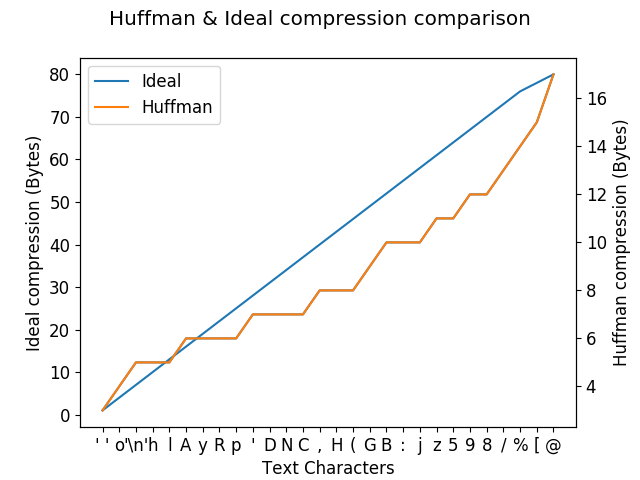
\includegraphics[width=0.48\textwidth]{experiments/huffman_idealness/huffman_idealness.png}
        \caption{Huffman-ideal compression comparison}
        \label{fig:huffman_idealness}
    \end{figure}



\end{document}
